\documentclass[
		paper=a4,
	  twoside=false,
	 fontsize=10pt,
			  titlepage,
			  plainheadsepline,
			  plainfootsepline,
			  headsepline,
			  footsepline,
		index=totoc,	% fügt Inhaltsverzeichnis in Inhaltsangabe ein
	   listof=totoc,	% fügt das Sourcenverzeichnis in Inhaltsangabe ein
 bibliography=totoc,	% fügt Literaturverzeichnis in Inhaltsangabe ein
	 abstract=false,		%needed?
	titlepage=false
]{scrreprt}

\raggedright

%\parskip2ex plus1ex minus0.5ex
\setlength{\parindent}{0.05\textwidth}

\usepackage[
		 left=3cm,
		right=3cm,
		  top=2.5cm,
	   bottom=2.5cm,
		includeheadfoot
]{geometry}

\usepackage[
		pdftex,
		colorlinks=true,
		 linkcolor=black,
		 citecolor=black,
		 filecolor=black,
		  urlcolor=black
]{hyperref}
\usepackage[all]{hypcap}

\usepackage[english, ngerman]{babel}\selectlanguage{ngerman}
\usepackage[ngerman]{translator}
\usepackage[acronym, toc, numberedsection=false]{glossaries}

\usepackage[utf8]{inputenc} %Kodierung, statt latin1 auch utf8 möglich
%\usepackage{setspace} \onehalfspacing

\usepackage{lmodern}
%\usepackage{ae,aeguill}
\usepackage{ae}

\usepackage{amsfonts}
\usepackage{amsmath}
\usepackage[automark]{scrpage2}
\pagestyle{scrheadings}
%\setlength{\headheight}{1.5\baselineskip}
\clearscrheadfoot

\usepackage[round,numbers,square]{natbib}
\bibliographystyle{alphadin}

\usepackage{graphicx}
\usepackage{epsfig}
\setlength{\unitlength}{10mm} %sets unitlength for picture-environment

\usepackage{rotating}
\usepackage{longtable}
\usepackage{multirow}
\usepackage{afterpage}

% \usepackage{eurosym} % euro sign

\usepackage{color}
\definecolor{blue}{rgb}{0.1647,0,1}
\definecolor{darkred}{rgb}{0.498,0,0.33333}
\definecolor{green}{rgb}{0.247,0.498,0.3725}
\definecolor{lightgray}{rgb}{0.95,0.95,0.95}

\usepackage{listings}
\lstset{
		language=Java,									% the language for the code
	escapeinside={(*@}{@*)},							% the comments in code that are not printed
	  basicstyle=\scriptsize\ttfamily\color{black},		% the style of the code font
	keywordstyle=\bfseries\color{darkred},				% the style for keywords
	 stringstyle=\color{blue},							% the style for strings
	commentstyle=\color{green},							% the style for comments
 identifierstyle=\color{black},							% the style for identifiers
		 numbers=left,									% where to put the line numbers
	 numberstyle=\tiny,									% the style of line numbers
showstringspaces=false,									% underline spaces in strings
	  stepnumber=1,										% the step between two numbered lines
	   numbersep=10pt,									% space between numbers and code
	  captionpos=b,										% where the caption should be printed (bottom)
		   frame=single,  								% if a frame should be printed around the code
		 tabsize=4,										% how many spaces one tab contains
       aboveskip=1cm,									% the space above the displayed listing
 backgroundcolor=\color{lightgray},							% background color to fill the listings with
			breaklines
}
% \renewcommand{\lstlistlistingname}{Quellcodeverzeichnis}
%\renewcommand{\baselinestretch}{1.5}\normalsize

% Schusterjungen/Hurenkinder ausschließen
\clubpenalty = 10000
\widowpenalty = 10000
\displaywidowpenalty = 10000

\newcommand{\figref}[1]{Abbildung~\ref{fig:#1}}
\newcommand{\secref}[1]{Abschnitt~\ref{sec:#1}}
\newcommand{\tabref}[1]{Tabelle~\ref{tbl:#1}}
\newcommand{\lstref}[1]{Listing~\ref{lst:#1}}
\newcommand{\srcref}[1]{Zeile~\ref{src:#1}}
\newcommand{\chpref}[1]{Kapitel~\ref{chp:#1}}
\newcommand{\icon}{icon~Systemhaus~GmbH\ }

% \usepackage{ifthen}
% \newcommand{\vgl}[2][]{% #1 = optional, #2 = notwendig
%   \ifthenelse{\equal{#1}{}}{
%        % Autor hat kein oder leeres optionales Argument angegeben
% 		(Vgl. \cite{#2})
%   }{%
%        % Autor hat optionales Argument angegeben
% 		(Vgl. \cite[#1]{#2})
%   }
% }
% \newcommand{\vglausf}[2][]{% #1 = optional, #2 = notwendig
%   \ifthenelse{\equal{#1}{}}{
%        % Autor hat kein oder leeres optionales Argument angegeben
% 		(Vgl. dazu ausführlich \cite{#2})
%   }{%
%        % Autor hat optionales Argument angegeben
% 		(Vgl. dazu ausführlich \cite[#1]{#2})
%   }
% }

\newcommand{\code}[1]{\texttt{#1}}
\newcommand{\notiz}[1]{\marginpar{\raggedright\tiny #1}}
\newcommand{\glentry}[3]{\newglossaryentry{#1}{name={#2},description={{#3}}}}

\newcommand{\md}{\emph{micro-debug}}
\newcommand{\mic}{\emph{Mic-1}}

\usepackage[texcoord]{eso-pic}
%\newcommand{\startprintinglogo}{
%	\AddToShipoutPicture{
%		\parbox[t]{\paperwidth}{
%			\vspace{0.5cm}
%			\hspace{16.2cm}
%			
\includegraphics[width=5.36cm,height=2.0cm]{includes/dhbw}
%		}
%	}
%}

\usepackage{syntax}
%\renewcommand{\notiz}[1]{} %uncomment for _NOT_ showing sidenotes!
\newcommand\thema{Design und Implementierung eines Debuggers für Mikro-Assembler-Programme}

\hypersetup{
	pdftitle={Studienarbeit}, pdfauthor={Christian Rösch, \icon},
	pdfsubject={\thema}, pdfkeywords={}
}

%\(i|c|o)head[plainpage]{otherpage} % i..links, o..rechts, c..zentriert
\ihead[Studienarbeit]{Studienarbeit}
\ohead[Christian Rösch]{Christian Rösch}
\ifoot[\rightmark]{\rightmark} 
\ofoot[\pagemark]{\pagemark} 

\loadglsentries{glossar}
\loadglsentries[\acronymtype]{abkuerzungen}
\makeglossaries

\begin{document}

	%\nocite{*} % Alle Einträge der .bib-Datei werden auch wenn unzitiert ins Literaturverzeichnis übernommen
	
	% don't write the text of these acronyms
	% \glsunset{asf}
	% \glsunset{html}

	\thispagestyle{empty}

\AddToShipoutPicture*{
	\parbox[t]{\paperwidth}{
		\vspace{2.0cm}
		\hspace{12.0cm}
		
\includegraphics[height=2.5cm]{includes/dhbw.jpg}
	}
}
\parbox[t]{\paperwidth}{}
\begin{center}
	\vspace{15mm}	{\LARGE\bf\thema}\\
	\vspace{20mm}	{\Large\textsc{Studienarbeit}}\\
	\vspace{15mm}	des Studiengangs Angewandte Informatik\\der Dualen Hochschule Baden-Württemberg Stuttgart\\
	\vspace{7,5mm}	von\\
	\vspace{7,5mm}	{\textbf{Christian Rösch}}\\
	\vspace{10mm}	Oktober 2011 - Mai 2012
\end{center}

\vfill

\begin{tabular*}{\textwidth}{p{7cm}l}
  \textbf{Bearbeitungszeitraum} &  Oktober 2011 - Mai 2012\\
  \textbf{Bearbeitungsdauer}    &  300~Stunden\\
  \textbf{Matrikelnummer}       &  0487930\\
  \textbf{Kurs}                	&  TIT09AIC\\
  \textbf{Ausbildungsfirma}     &  \icon{} -- Stuttgart\\
  % \textbf{Gutachter der Ausbildungsfirma} &  Dipl.-Inf. Steffen Huber\\
  \textbf{Gutachter der Studienakademie} & Prof.~Dr.~Karl~Stroetmann\\
\end{tabular*}\clearpage

	\pagenumbering{roman}
% 	\include{Erklaerung}\clearpage

%	\startprintinglogo
 	\chapter*{Einleitung}
Die vorliegende Arbeit stellt \md vor, den Debugger für den CISC-Prozessor, der in \cite{Tanenbaum1998} vorgestellt wird: \mic.

Im Gegensatz zu einem RISC-Prozessor sind die Maschinenbefehle in der \mic nicht in Hardware implementiert, sondern werden durch einen Mikroprogramm-Speicher definiert. Dieser wird in Mikro-Assembler programmiert und ermöglicht es Maschinenbefehle auf einem hohen Abstraktionsniveau zu definieren und ohne Veränderung der Hardware anzupassen.

\section*{Aufgabenstellung}
Im Skript der Vorlesung Rechnertechnik \notiz{Verweis auf Skript der VL Rechnertechnik einfügen} wurde ein Mikro-Assembler für die \mic vorgestellt. Ziel dieser Arbeit istder Entwurf und die Implementierung eines Debuggers für diesen Mikro-Assembler. Der Debugger soll die Entwicklung von Mikro-Assembler- und Assembler-Programmen für die \mic erleichtern.

Um entsprechenden Mikro-Assembler- und Assembler-Bytecode debuggen zu können, ist es nötig die \mic zu simulieren. Im Jahr 2004 wurde von Thomas Kutzer eine Studienarbeit zum Thema ``Mic-1 Simulator'' verfasst.\notiz{Verweis einfügen!?} Der Debugger soll den darin entwickelten Simulator ersetzen und um einige Funktionen ergänzen.

In der Arbeit sollen dabei hauptsächlich zwei Teilaufgaben bearbeitet werden.

\subsection*{Debugger für die Konsole}
Zunächst soll eine Version des Debuggers entwickelt werden, der über die Konsole bedient wird. Das Ziel dabei ist eine Implementierung des Debuggers unabhängig von der Darstellung der Ein- und Ausgabe.

Der Debugger soll in der Lage sein zwei Binärdateien einzulesen: eine Datei, die den Mikro-Assembler enthält und eine, die den Assembler-Code enthält. Der Assembler-Code soll grundsätzlich frei wählbar sein, als Referenz für diese Arbeit soll aber der IJVM-Assembler dienen.

Der Benutzer soll Breakpoints (Haltepunkte) definieren können, die die Simulation des Mikro-Assembler-Programms unterbrechen. Hierbei soll der Benutzer die Möglichkeit bekommen, Breakpoints für bestimmte Mikro-Assembler-Instruktionen aber auch für bestimmte Assembler-Instruktionen zu definieren.

Die Werte ausgewählter Register sollen vom Benutzer sowohl angezeigt, als auch überwacht werden können -- ebenso der Inhalt des Stacks.

\subsection*{GUI für den Debugger}
Im zweite Teil der Aufgabe soll für den entwickelten Debugger eine grafische \notiz{graphisch/grafisch} Oberfläche entwickelt werden.

Die grafische Oberfläche soll sowohl den Mikro-Assembler als auch den Assembler anzeigen. Auch die Register mit ihren Werten und der Stack soll sichtbar sein.

Die grafische Oberfläche soll dem Benutzer ermöglichen, Breakpoints über die Oberfläche zu setzen. Außerdem soll dem Benutzer angezeigt werden, welcher Mikro-Assembler- und Assembler-Befehl gerade abgearbeitet wird.

Da in dieser Arbeit ein allumfassender Debugger weder geschaffen werden kann noch soll, ist besonders darauf zu achten, die Wartung und Erweiterung des Debuggers Außenstehenden Personen zu ermöglichen. Besonders der zu schreibende Code soll daher gut dokumentiert werden; beispielsweise andere Studenten sollen sich in den Code einarbeiten können und neue Funktionalitäten implementieren oder bestehende Funktionalitäten anpassen können.

\section*{Aufbau der Arbeit}
Die Arbeit ist in zwei Teile geteilt: Im ersten Teil wird die Bedienung und im zweiten Teil wird die Entwicklung des \md erläutert.

\subsection*{Bedienung}
Im \chpref{allgemein} wird der \md allgemein beschrieben: Welche Systemvoraussetzungen gelten, wie man den \md konfiguriert und wie er in andere Sprachen übersetzt werden kann. Außerdem wird beschrieben, wie man die Log-Ausgaben des \md nutzen und konfigurieren kann.

Die Bedienung des \md in der Konsolenvariante wird im \chpref{bed-konsole} beschrieben; Es werden die Parameter des \md erklärt, die verschiedenen Befehle erläutert und ein Beispiel gezeigt, wie ein Fehler mit dem Debugger gefunden werden kann.

Im \chpref{bed-gui} wird die grafische Oberfläche beschrieben; Es werden die Unterschiede zur Konsolenvariante genannt, die verschiedenen Oberflächenelemente erklärt und ein Beispiel gezeigt, wie ein Fehler mit dem Debugger mit grafischer Oberfläche gefunden werden kann.

\subsection*{Entwicklung}
Im \chpref{werkzeuge} werden einige Werkzeuge beschrieben, die zur Entwicklung des \md genutzt wurden und deren Verständnis nötig ist, um selbst Änderungen am Projekt vorzunehmen. In \chpref{entw-allg} gehe ich kurz auf die Notwendigkeit der automatisierten Tests ein.

Die nachfolgenden Kapitel beschreiben, welche Funktionalität des \md durch welche Klassen erledigt werden. \chpref{prozessor} gibt einen Überblick über die Simulation der \mic und zeigt welcher Code die jeweilige Hardwarekomponente repräsentiert. Im \chpref{konsole} wird der Coder für die Konsolenvariante und in \chpref{gui} der Code für die grafische Oberfläche erklärt.\clearpage
	\tableofcontents\clearpage
	\printglossary\clearpage
	\printglossary[type=\acronymtype, title={Abkürzungsverzeichnis}, toctitle={Abkürzungsverzeichnis}]\clearpage
	\listoffigures\clearpage
	%\listoftables\clearpage
	\lstlistoflistings\clearpage
	\pagenumbering{arabic}

	\part{Bedienung}
\chapter{Allgemein}
\chplbl{allgemein}
Sowohl die Konsolenvariante als auch die grafische Oberfläche des \md{} benötigen keine Installation; sie werden beide als \texttt{.zip}-Archiv heruntergeladen und sind direkt nach dem Entpacken nutzbar. Die Datei heiß üblicherweise \texttt{micro-debug-version.zip} und enthält mehrere Dateien:

\begin{description}
\item[micro-debug-version.jar] enthält den Programmcode des Debuggers und kann mit dem Befehl \texttt{\$ java -jar} ausgeführt werden.\notiz{Debugger und \md{} synonym verwenden?}
\item[micro-debug.sh und micro-debug.bat] sind die Startskripte des \md{} für Windows und Linux. Der \md{} kann durch Ausführen dieser Skripte gestartet werden -- der Benutzer muss sich dadurch nicht um die Konfiguration des Klassenpfades kümmern. Die Startskripte sind so geschrieben, dass sie von beliebigen Orten ausgeführt werden können. Der Benutzer kann den Debugger also von vielen Arbeitsverzeichnissen aus aufrufen und hat die Konfigurationsdateien nur an einer Stelle zu pflegen.
\item[config/micro-debug.properties] ist die Konfigurationsdatei für den \md{}, hier kann beispielsweise die Größe des Hauptspeichers konfiguriert werden -- siehe \secref{konfiguration}.
\item[config/logging.properties] ist die Konfigurationsdatei für das Logging des \md{} -- hier kann der Benutzer definieren, ob und welche Ausgaben auf der Konsole oder in einer Datei erscheinen sollen -- siehe \secref{logs}.
\item[config/lang/] enthält die Textressourcen des \md{} -- siehe \secref{lokalisierung}.\notiz{Ressource/Resource?}
\item[lib/] enthält die verwendeten Bibliotheken, zur Zeit nur in der \mdg{} verwendet.
\end{description}

\section{Systemvoraussetzungen}
\seclbl{systemvoraussetzungen}
Der \md{} ist in Java geschrieben und daher prinzipiell an keine spezielle Plattform gebunden. Voraussetzung für die Nutzung des \md{} ist lediglich Java~5.

In der Praxis differenzieren sich die verschiedenen Plattformen, auf denen Java verfügbar ist, in einigen Feinheiten. Daher ist es prinzipiell möglich, dass sich der \md{} auf gewissen Plattformen nicht wie gewünscht verhält. Wie anhand der Startskripte zu erkennen ist, wurde der \md{} im Blick auf Linux und Windows entwickelt und darauf getestet; um den \md{} auf einer weiteren Plattform zu nutzen, muss zumindest das Startskript eigenständig geschrieben werden.

Die Konsolenvariante nutzt bislang einen Thread, die Version des \md{} mit grafischer Oberfläche mindestens zwei (wie Kapitel/Abschnitt X beschrieben\notiz{Verweis auf Kapitel einfügen}), die allerdings selten parallel arbeiten. Für die Ausführungsgeschwindigkeit des \md{} ist die Anzahl der verfügbaren Prozessorkerne daher irrelevant.

\section{Konfiguration}
\seclbl{konfiguration}
Wie oben bereits angedeutet findet die Konfiguration des \md{} in \datei{properties}en statt. Die Konfigurationsdatei für den \md{} ist die Datei \texttt{config/micro-debug.properties} -- wie in \datei{properties}en üblich, werden hier Key/Value\notiz{Key/value!?}-Paare hinterlegt.

\begin{lstlisting}[language=sh,caption={Eintrag in \texttt{conf/micro-debug.properties}},label=\lstlbl{md-props-entry}]
# default value for the register CPP
mic1.register.cpp.defval = 0x4000
\end{lstlisting}

\lstref{md-props-entry} zeigt einen beispielhaften Eintrag in der Konfigurationsdatei: Den Startwert für das Register CPP\notiz{Register Befehl erstellen?}. Diese Datei kann für jeden Schlüssel genau einen Wert enthalten, ist für einen Schlüssel kein Wert konfiguriert oder ist ein ungültiger Wert konfiguriert, nutzt der Debugger den Standardwert für den jeweiligen Schlüssel.\notiz{Prüfen und ggf. einfügen, dass fallback anständig geloggt wird und das dann hier auch erwähnen.}

Dadurch ist es möglich ein Update des \md{} durch die Ersetzung der \datei{jar} zu realisieren. Denn vom Benutzer geänderte Werte müsste er in der neuen Version wieder mühsam nachpflegen; das Nutzen von Standardwerten bei fehlenden Konfigurationseinträgen ermöglicht es dem Benutzer seine persönliche Konfigurationsdatei von Version zu Version des \md{} zu behalten.\notiz{Überlegen, ob nicht irgendwo ein Update-Abschnitt sinnvoll ist}

\subsection{Zahlenformat}
\seclbl{zahlenformat}
\notiz{Wahrscheinlich ist es sinnvoll in den properties Dateien einzutragen, von welchem Typ ein Schlüssel sein soll und dies dann hier auch zu notieren}.
In \lstref{md-props-entry} ist zu sehen, wie dem Register CPP der Standardwert \texttt{0x4000} zugewiesen wird -- hier hexadezimal notiert. Andere Konfigurationseinträge sind dezimal eingetragen; welches Zahlenformat ist nun wo anzuwenden?

Für den \md{} ist es irrelevant, welches Zahlenformat bei welchem Eintrag verwendet wird. Er parst die gegebene Zahl und wandelt sie in ein Integer um, dadurch kann der Benutzer für jeden Eintrag das passende Zahlenformat wählen.

Welche Zahlenformate gibt es außer dezimal und hexadezimal? Der \md{} unterstützt alle Zahlensysteme mit der Grundzahl von $b=2$ bis $b=36$. Generell werden die Zahlen in der Art \texttt{ZAHL\_BASIS} angegeben -- \texttt{ZAHL} wird in dem jeweiligen Zahlensystem und \texttt{BASIS} im Dezimalsystem angegeben.

Für die wohl am häufigsten verwendeten Zahlensysteme gibt es die in \tabref{vereinfachungen-zahlenformate} dargestellten Vereinfachungen -- diese Vereinfachungen sind aber nicht verpflichtend, sowohl \texttt{A\_16} als auch \texttt{0xA} ist zulässig.

\begin{table}[h]
  \centering
  \begin{tabular}[h]{|lll|}
    \hline
    Zahlensystem      & ausführlich      & vereinfacht     \\
    \hline
    Dualsystem        & \texttt{1010\_2} & \texttt{0b1010} \\
    Oktalsystem       & \texttt{12\_8}   & \texttt{0o12}   \\
    Dezimalsystem     & \texttt{10\_10}  & \texttt{10}     \\
    Hexadezimalsystem & \texttt{A\_16}   & \texttt{0xA}    \\
    \hline
  \end{tabular}
  \caption{Vereinfachungen typischer Zahlenformate im \md{}}
  \tablbl{vereinfachungen-zahlenformate}
\end{table}

\subsection{Logs}
\seclbl{logs}
Im Optimalfall ist sowohl der \md{} als auch der Benutzer fehlerfrei. Da dies in der Praxis selten beobachtet wird, ist oftmals Fehleranalysen nötig. Log-Ausgaben protokollieren vermeintlich wichtige Vorgänge für solche Analysen und sind daher ein guter Ansatzpunkt, um die Fehlerursache zu finden.

Der \md{} wird im Startskript so gestartet, dass die Log-Konfiguration aus der Datei \texttt{conf/logging.properties} genutzt wird. Die genaue Syntax und Semantik der Konfigurationseinträge ist hier und hier \notiz{TODO} beschrieben.
% http://docs.oracle.com/javase/1.5.0/docs/guide/logging/overview.html
% http://www.vogella.com/articles/Logging/article.html

Standardmäßig werden von \md{} alle Log-Ausgaben mit der Wichtigkeit \texttt{INFO} oder höher in Dateien geschrieben, die im home-Verzeichnis des Benutzers liegen. Die verschiedenen Log-Level sind von wichtig absteigend \texttt{SEVERE}, \texttt{WARNING}, \texttt{INFO}, \texttt{CONFIG}, \texttt{FINE}, \texttt{FINER} und \texttt{FINEST}.

\subsection{ijvm.conf}
\seclbl{ijvm-conf}
Der \md{} ist so konstruiert, dass er theoretisch für beliebige Assembler als Debugger dienen kann. Allerdings wird der \md{} in der Praxis wohl vorwiegend mit IJVM-Assembler genutzt. Um diesen Assembler disassemblieren zu können, gibt es eine Konfigurationsdatei -- die \texttt{ijvm.conf}. Damit der \md{} einen gewissen Standardsatz an Befehlen versteht, wird diese Datei im \texttt{.jar}-Archiv ausgeliefert.

Möchte der Benutzer diese Datei anpassen genügt es, die neue Version der Datei im Verzeichnis \texttt{conf/} abzulegen; durch das Startskript wird sie dann auf dem Klassenpfad vor der entsprechenden Datei im \texttt{.jar}-Archiv geladen und ersetzt diese somit.

Die Datei ist zeilenweise zu lesen, wobei eine Zeile nach folgendem Format aufgebaut ist.

\setlength{\grammarparsep}{3pt plus 1pt minus 1pt}
\setlength{\grammarindent}{10em} % increase separation between LHS/RHS 
\begin{grammar}

<line>     ::= <comment>
  \alt         <address> <white>+ <identifier> <white>* <argumentlist> <comment>?

<comment>  ::= '//' <text>

<address> ::= '0x' <hexchar> <hexchar>

<hexchar> ::= '0' | '1' | '2' | '3' | '4' | '5' | '6' | '7' | '8' | '9' | 'A' | 'B' | 'C' | 'D' | 'E' | 'F'

<identifier> ::= <word>

<argumentlist> ::= ( <white> <argument> <white>* )*

<argument> ::= 'byte' | 'const' | 'index' | 'label' | 'offset' | 'varnum'

<white>    ::= ' ' | '$\backslash$t'
\end{grammar}

\section{Lokalisierung}
\seclbl{lokalisierung}
Die Ausgaben des \md{} wurden in Englisch geschrieben -- weitere Sprachen können leicht über das Verzeichnis \texttt{conf/lang/} hinzugefügt werden.

In diesem Verzeichnis liegen verschiedene \datei{xml}, die dazu dienen, dem Benutzer Ausgaben in seiner Landessprache anzuzeigen. Die Sprache, die der Benutzer angezeigt bekommt, hängt von der Locale-Einstellung des Computers ab.

Der \md{} sucht dann für diese Sprache folgende vier Dateien, die Key/Value-Paare für die Textkonstanten enthalten:
\begin{description}
\item[text_lang_CT_var1.xml] wobei \emph{lang} die Sprache, \emph{CT} die Länderkennung und \emph{var1} die Variante ist, die vom Locale gegeben sind. Diese Datei ist die spezifischste und wird zuerst geladen (sofern sie existiert). Schlüssel, die hier nicht gefunden werden, werden in den folgenden Dateien gesucht.
\item[text_lang_CT.xml]
\item[text_lang.xml]
\item[text.xml] die Basis-Datei für die Internationalisierung. Wenn ein Schlüssel bisher noch nicht gefunden wurde oder die anderen Dateien nicht existieren, dann wird er in dieser Datei gesucht.
\end{description}

Der Aufbau dieser vier Dateien ist hierarschich, ein Schlüssel, der in der spezifischsten Datei gefunden wurde, wird aus den anderen Dateien nicht mehr ausgewertet. Anhand eines Beispiels soll diese Funktionalität genauer erläutert werden:

Gegeben seien die drei Dateien aus \lstref{locale-file-de-de}, \lstref{locale-file-de} und \lstref{locale-file}. \lstref{locale-result} zeigt das Ergebnis nach der Auswertung dieser drei Dateien. Es ist zu sehen, wie die Einträge sich überschreiben -- ein Benutzer mit englischem Locale würde in diesem Beispiel den Eintrag für \texttt{border2} nicht erhalten und hätte dafür keinen definierten Wert.

Die Reihenfolge der Key/Value-Paare ist willkürlich und kann beliebig verändert werden.

\begin{lstlisting}[language=XML,caption={Beispiel für Datei \texttt{text_de_DE.xml}},label=\lstlbl{locale-file-de-de}]
<?xml version="1.0" encoding="UTF-8"?>
<!DOCTYPE properties SYSTEM "http://java.sun.com/dtd/properties.dtd">
<properties>
	<entry key="border">+*+*+*+*+*</entry>
	<entry key="border2">---</entry>
</properties>
\end{lstlisting}

\begin{lstlisting}[language=XML,caption={Beispiel für Datei \texttt{text_de.xml}},label=\lstlbl{locale-file-de}]
<?xml version="1.0" encoding="UTF-8"?>
<!DOCTYPE properties SYSTEM "http://java.sun.com/dtd/properties.dtd">
<properties>
	<entry key="file-not-found">Datei nicht gefunden {0}</entry>
	<entry key="version">Micro-Debug - Version {0}</entry>
</properties>
\end{lstlisting}

\begin{lstlisting}[language=XML,caption={Beispiel für Datei \texttt{text.xml}},label=\lstlbl{locale-file}]
<?xml version="1.0" encoding="UTF-8"?>
<!DOCTYPE properties SYSTEM "http://java.sun.com/dtd/properties.dtd">
<properties>
	<entry key="version">Micro-Debug: Version {0}</entry>
	<entry key="file-not-found">file not found {0}</entry>
	<entry key="border">----------------------------------------</entry>
</properties>
\end{lstlisting}

\begin{lstlisting}[language=XML,caption={Beispiel für Ergebnis nach Verarbeitung der Lokalisierungsdateien},label=\lstlbl{locale-result}]
<?xml version="1.0" encoding="UTF-8"?>
<!DOCTYPE properties SYSTEM "http://java.sun.com/dtd/properties.dtd">
<properties>
	<entry key="version">Micro-Debug - Version {0}</entry>
	<entry key="file-not-found">Datei nicht gefunden {0}</entry>
	<entry key="border">+*+*+*+*+*</entry>
	<entry key="border2">---</entry>
</properties>
\end{lstlisting}

Dieses System ermöglicht das einfache Hinzufügen neuer Sprachen -- dieser Vorgang ist nicht für den Benutzer vorgesehen, aber prinzipiell kann er in diesen Dateien Anpassungen vornehmen und sich dadurch die Ausgaben an seine Bedürfnisse anpassen.

Im Gegensatz zur Konfigurationsdatei gibt es hier allerdings kein Fallback, sodass fehlende Werte mit einem Fehlertext belegt werden. Die Übersetzungsdateien bedürfen nach einem Update daher womöglich größerer Überarbeitungen, wenn der Benutzer seine Anpassungen behalten möchte.

Die Werte können Platzhalter enthalten. Platzhalter gelten nur für ein bestimmtes Key/Value-Paar und sind von null beginnend nummeriert in der Form \texttt{{0}} zu verwenden. Der Inhalt mit dem der Platzhalter gefüllt wird kann in den Kommentaren in der Datei nachgelesen werden.

Zusätzlich zu den \texttt{text...xml}-Dateien gibt es bei der grafischen Oberfläche des \md{} auch \texttt{text-gui...xml}-Dateien, die die Textkonstanten für die grafische Oberfläche enthalten.

Die Log-Ausgaben sind immer auf Englisch und können über die \datei{xml} nicht verändert werden.
\chapter{Interaktion per Konsole}
\chplbl{bed-konsole}
Wie in \chpref{allgemein} beschrieben, muss der \md nicht installiert werden: Vom Herunterladen bis zum Starten des \md genügen folgende Schritte.

\begin{enumerate}
\item Die Datei \texttt{micro-debug-version.zip} von der Projektseite \cite{Roesch2012} herunterladen
\item Die \datei{zip} in ein beliebiges Verzeichnis entpacken (beispielsweise \texttt{/opt/micro-debug/})
\item Das Verzeichnis des \md dem \texttt{PATH} hinzufügen
\item Den \md starten -- mit \texttt{micro-debug.sh~-{}-help}
\end{enumerate}

Der \md kann durch einige Parameter gesteuert werden und wird nach dem Start durch Befehle bedient. Ich werde daher zunächst die verschiedenen Parameter des \md und dann die Befehle zur Bedienung des \md erklären. Am Ende des Kapitels zeige ich in einem Tutorial, wie mit dem \md Fehler im \ac gefunden werden können.

\section{Parameter}
Der Standardaufruf für den \md ist in \lstref{aufruf-konsolenversion} zu sehen. Es gibt zwei verpflichtende Parameter: Die Pfade zur \ma und zur \ac -Datei\notiz{Irgendwo den Aufbau der beiden Dateien erwähnen}. Die beiden Pfade können sowohl relativ als auch absolut angegeben werden, wichtig ist allerdings, dass zuerst der Pfad zur \ma und dann der Pfad zur \ac -Datei angegeben wird. Werden die beiden Pfade vertauscht, so startet der \md nicht und bricht mit einer Fehlermeldung ab.

\begin{lstlisting}[language=sh,caption={Aufruf des \md},label=\lstlbl{aufruf-konsolenversion}]
micro-debug.sh [PARAMETER]... MIC1 IJVM
\end{lstlisting}

Neben den beiden Dateipfaden gibt es im Folgenden erklärte optionale Parameter. Jeder Parameter kann sowohl in der langen (mit doppeltem Minus) als auch in der kurzen (einfaches Minus gefolgt von einem Zeichen) Variante angegeben werden.

\begin{description}
\item[-h, -{}-help]
  ist dieser Parameter gegeben, so wird die Hilfe angezeigt, die neben den verschiedenen Aufrufmöglichkeiten die möglichen Parameter erklärt. Zusätzlich werden noch einige andere Informationen angezeigt, wie beispielsweise Kontaktmöglichkeiten oder ein Hinweis, wo Fehler berichtet werden können.

\item[-o, -{}-output-file FILE]
  wenn dieser Parameter angegeben ist, so wird die Ausgabe der \mic (nicht des \md) in eine Datei umgelenkt. Normalerweise wird die Ausgabe der \mic auf der Konsole ausgegeben.

  Das Argument \texttt{FILE} ist der Pfad zur Datei, in die die Ausgabe geschrieben werden soll. Wenn die Datei bereits existiert, wird die Ausgabe an das Ende der Datei angehängt.

  Unter Linux kann man dann in einer zweiten Konsole diese Datei beispielsweise mit \texttt{tail~-f} anzeigen und die Ausgabe der \mic komfortabel von der Ausgabe des \md trennen. In diesem Szenario ist auch der Parameter \texttt{-{}-unbuffered-output} sinnvoll.

\item[-u, -{}-unbuffered-output]
  verhindert die Pufferung der Ausgabe der \mic. Normalerweise gibt der \md die Ausgabe der \mic zeilenweise aus, also erst bei der Ausgabe eines Zeilenumbruchs. Verwendet man den Parameter \texttt{-{}-output-file} oder möchte man aus sonstigen Gründen jedes ausgegebene Zeichen der \mic direkt auf der Konsole sehen, so ist dieser Parameter die Lösung.

  \emph{Vorsicht!} Wird dieser Parameter ohne \texttt{-{}-output-file} genutzt, so kann ist es schwer, die ausgegebenen Zeichen der \mic ausfindig zu machen, da sie in der Menge der Ausgaben des \md untergehen.

\item[-v, -{}-version]
  gibt die Version des \md aus.
\end{description}

Wenn einer der Parameter \texttt{-{}-help} oder \texttt{-{}-version} angegeben wurde, startet der \md nicht. Dies kann genutzt werden, um ohne vorhandene Bytecode-Dateien Informationen über den \md anzeigen zu können. \lstref{aufrufe-ohne-start} zeigt, wie der \md daher ohne Bytecode-Dateien aufgerufen werden kann.

\begin{lstlisting}[language=sh,caption={Aufruf des \md ohne Start},label=\lstlbl{aufrufe-ohne-start}]
micro-debug.sh --help
micro-debug.sh --version
\end{lstlisting}

Bei der Abarbeitung der gegebenen Parameter hängt die Reihenfolge der Parameter nicht von der Reihenfolge ab, in der sie dem \md als Parameter übergeben wurden. Wichtig ist nur, dass die beiden Bytecode-Dateien die letzten beiden Parameter und in der richtigen Reihenfolge aufgeführt sind.

\section{Befehle}
Bei der Bedienung des \md muss der Benutzer zwischen den verschiedenen Befehlen auch Zeichen für die \mic eingeben. Damit der Benutzer sieht, ob die Eingabe für den \md oder die \mic sind, gibt der \md '\texttt{micro-debug> }' und die \mic '\texttt{mic1> }' aus, bevor eine Eingabe erwartet wird. Wenn die \mic eine Eingabe erwartet, kann der Benutzer mehrere Zeichen auf einmal eingeben -- an die \mic werden die eingegebenen Zeichen plus ein Zeilenumbruch gesendet. Sollte der \ac einzelne Zeichen in einer Schleife einlesen, sollte die gesamte Zeile daher auf einmal eingeben werden.

Ist der \md gestartet lässt er sich durch verschiedene Befehle bedienen, die ich jetzt ausführlich beschreiben werde.

Die verschiedenen Befehle können ein oder mehrere Argumente benötigen. Die Argumente haben einen der folgenden Datentypen:
\begin{description}
\item[Register] ist der Name eines Registers, also \reg{CPP}, \reg{H}, \reg{LV}, \reg{MAR}, \reg{MBR}, \reg{MBRU}, \reg{MDR}, \reg{OPC}, \reg{PC}, \reg{SP} oder \reg{TOS}.
\item[Zahl] ist eine Zahl im Wertebereich eines \emph{Integers}\notiz{Verweis?}. Die Formate für die Eingabe der Zahl habe ich in \secref{zahlenformat} beschrieben.
\end{description}

Je nach Befehl kann der zulässige Wertebereich eingeschränkt sein -- eine solche Einschränkung ergibt sich aus der Beschreibung des jeweiligen Befehls.

\begin{description}
\item[break] \emph{Register [Zahl]}

  setzt einen Breakpoint für das gegebene \emph{Register}: Sobald das Register den Wert \emph{Zahl} erhält, hält der \md an. Der \md hält, \textbf{nachdem} das Register den Wert erhalten hat -- da dies unter Umständen zu spät ist, gibt es die Möglichkeit, das Argument \emph{Zahl} wegzulassen. Wird nur ein Register (ohne Wert) angegeben, hält der \md \textbf{bevor} das Register einen neuen Wert zugewiesen bekommt.

\item[exit] \hspace*{\fill}\\

  beendet den \md.

\item[help] \hspace*{\fill}\\

  zeigt die verfügbaren Befehle mit einer kurzen Beschreibung an. Zeigt des weiteren einige Zusatzinformationen über den \md an.

\item[ls-break] \hspace*{\fill}\\

  zeigt alle Breakpoints mit der jeweiligen Bedingung an. Jeder Breakpoint erhält eine Identifikationsnummer, die bei anderen Operationen, wie dem Entfernen, angegeben werden muss.

\item[ls-macro-code] \emph{[Zahl1 [Zahl2]]}

  zeigt den disassemblierten \ac an. Dabei gibt es drei mögliche Konstellationen der Parameter:
  \begin{itemize}
  \item Wird \textbf{kein Parameter} gegeben, wird der vollständige \ac angezeigt.
  \item Wird \textbf{ein Parameter} \emph{Zahl1} gegeben, wird die angegebene Anzahl an Zeilen vor und nach der aktuellen Zeile angezeigt.
  \item Werden \textbf{zwei Parameter} gegeben, wird der \ac von Zeile \emph{Zahl1} bis zur Zeile \emph{Zahl2} (inklusive) angezeigt.
  \end{itemize}

  Da der \md nur den Bytecode kennt, gibt es eigentlich keine Zeilen. Der \md schreibt pro Zeile einen Befehl (inklusive Argumente), somit existieren Zeilennummern, die für den \md als Referenz dienen.

\item[ls-micro-code] \emph{[Zahl1 [Zahl2]]}

  zeigt den disassemblierten \mac an und arbeitet wie \texttt{ls-macro-code}. Es gibt drei mögliche Konstellationen der Parameter:
  \begin{itemize}
  \item Wird \textbf{kein Parameter} gegeben, wird der vollständige \mac angezeigt.
  \item Wird \textbf{ein Parameter} \emph{Zahl1} gegeben, wird die angegebene Anzahl an Zeilen vor und nach der aktuellen Zeile angezeigt.
  \item Werden \textbf{beide Parameter} gegeben, wird der Mikro-Assembler-Code von Zeile \emph{Zahl1} bis zur Zeile \emph{Zahl2} (inklusive) angezeigt.
  \end{itemize}

  Wie bei \texttt{ls-macro-code} schreibt der \md pro Zeile eine \mai (die $36~Bit$, die die Instruktion spezifizieren), somit existieren Zeilennummern, die für den \md als Referenz dienen.

\item[ls-mem] \emph{Zahl1 Zahl2}

  zeigt den Inhalt des Hauptspeichers zwischen den Adressen \emph{Zahl1} und \emph{Zahl2} (inklusive) an. Die Adressen des Hauptspeichers sind Wortadressen -- jedes Wort hat eine Größe von $32~Bit$.

\item[ls-reg] \emph{[Register]}

  zeigt den Wert von dem gegebenen \emph{Register} an; wird das optionale Argument weggelassen, werden alle Register und deren Werte angezeigt.

\item[ls-stack] \hspace*{\fill}\\

  zeigt den aktuellen Stack an.

  \emph{Hinweis:} Dieser Befehl wird durch die Konfigurationsoption \texttt{stack.elements.to.hide} beeinflusst. Normalerweise wird der Stack von dem initialen Stackpointer bis zum aktuellen Stackpointer ausgegeben. Da dies unter Umständen mehr Elemente liefert, als der Stack tatsächlich enthält, gibt es die Möglichkeit über die Konfiguration die Ausgabe der ersten Elemente zu unterdrücken.

Möchte man den realen (im Speicher vorhandenen) Stack sehen, sollte man sicherstellen, dass \texttt{stack.elements.to.hide = 0} konfiguriert ist.

\item[macro-break] \emph{Zahl}

  fügt einen Breakpoint hinzu, der den \md anhält, sobald der \ac an der Adresse \emph{Zahl} ausgeführt werden soll. \emph{Adresse} muss Element aus der Menge der von \texttt{ls-macro-code} angezeigten Zeilennummern sein.

\item[micro-break] \emph{Zahl}

  fügt einen Breakpoint hinzu, der den \md anhält, sobald der \mac an der Adresse \emph{Zahl} ausgeführt werden soll. \emph{Adresse} muss Element aus der Menge der von \texttt{ls-micro-code} angezeigten Zeilennummern sein.

\item[micro-step] \emph{[Zahl]}

  führt die nächsten \emph{Zahl} \mais aus; wird kein Argument gegeben, so wird eine \mai ausgeführt.

\item[reset] \hspace*{\fill}\\

  die \mic wird in den Anfangszustand zurückgesetzt: Der Hauptspeicher und die Register werden auf die initialen Werte zurückgesetzt. Auch die Ein- und Ausgabe der \mic wird geleert. Die Informationen des \md, vor allem die Breakpoints, bleiben allerdings erhalten und müssen vom Benutzer nicht erneut gesetzt werden.

\item[rm-break] \emph{Zahl}

  entfernt den Breakpoint mit der Nummer \emph{Zahl}. Die Nummer des Breakpoints ist die Identifikationsnummer, die mit \texttt{ls-break} angezeigt wird.

\item[run] \hspace*{\fill}\\
  
  führt alle Instruktionen bis zum Programmende oder bis zum nächsten Breakpoint aus.

  \emph{Hinweis:} Unter Umständen und ungünstigem Programmcode kann das zu debuggende Programm in eine Schleife geraten, welche ohne Breakpoints nur durch den Programmabbruch verlassen werden kann.

\item[set] \emph{Register Zahl}

  weist dem \emph{Register} den Wert \emph{Zahl} zu.

\item[set-mem] \emph{Zahl1 Zahl2}

  schreibt den Wert \emph{Zahl2} an die Wortadresse \emph{Zahl1} im Hauptspeicher.

  \emph{Hinweis:} Auch wenn dieser Befehl offensichtlich dazu genutzt werden könnte den \ac zu manipulieren, ist er für diesen Zweck nicht vorgesehen.

\item[step] \emph{[Zahl]}

  führt die nächsten \emph{Zahl} \ais aus; wird kein Argument gegeben, so wird eine \ai ausgeführt.

\item[trace-mac] \hspace*{\fill}\\
  
  der \ac wird nun beobachtet. Dadurch wird jede \ai angezeigt, nachdem sie ausgeführt wurde.

\item[trace-mic] \hspace*{\fill}\\

  der \mac wird nun beobachtet. Dadurch wird jede \mai angezeigt, nachdem sie ausgeführt wurde.

\item[trace-reg] \emph{[Register]}

  das gegebene \emph{Register} wird nun beobachtet. Dadurch wird der Wert des Registers angezeigt, wenn er sich ändert. Wird das optionale Argument weggelassen, werden alle \emph{Register} beobachtet.

\item[trace-var] \emph{Zahl}

  die Variable \emph{Zahl} wird nun beobachtet. Dadurch wird der Inhalt der Variable angezeigt, wenn er sich ändert.

  \emph{Zahl} ist die Nummer der lokalen Variable. Wird eine Methode im \ac aufgerufen, ändert sich der Zeiger \reg{LV} und damit auch die Identität der lokalen Variablen. Wird also Variable Nummer~1 in Methode X beobachtet und führt der \md gerade Methode Y aus, wird eine Änderung der jetzigen lokalen Variable~1 nicht ausgegeben (sofern diese nicht auch beobachtet wird).

\item[untrace-mac] \hspace*{\fill}\\
  
  beendet das Beobachten des \ac. Dadurch werden ausgeführte \ai nun nicht mehr ausgegeben.

\item[untrace-mic] \hspace*{\fill}\\

  beendet das Beobachten des \mac. Dadurch werden ausgeführte \mai nun nicht mehr ausgegeben.

\item[untrace-reg] \emph{[Register]}

  beendet das Beobachten des angegebenen \emph{Register}s. Wird das optionale Argument weggelassen, wird nun kein Register mehr beobachtet.

\item[untrace-var] \emph{Zahl}

  beendet das Beobachten der lokalen Variable Nummer \emph{Zahl}.
\end{description}

\section{Tutorial}
\seclbl{tutorial-konsole}
In diesem Abschnitt möchte ich ein Tutorial beschreiben, um in das Arbeiten mit dem \md einzuführen. Ich beschreibe das Debuggen eines Assembler-Programms: ein Programm zum Einlesen von Binärzahlen. \lstref{binary-read-c} zeigt den Code für das Programm in C\notiz{C referenz? erklärn?} und soll hier als Verständnis des Algorithmus dienen.

\begin{lstlisting}[language=c,caption={C-Programm zum Einlesen einer Binärzahl},label=\lstlbl{binary-read-c}]
int main() {
  int character = 0;
  int result = 0;
  while(1) {
    character = getchar();
    if( c == '\n' ) {
      return result;
    }
    c = c - '0';
    result = 2 * result + c;
  }
}
\end{lstlisting}

Der entsprechende \ac ist in \lstref{binary-read-jas} aufgeführt. Dieses Programm muss nun kompiliert werden -- \name{Ontko} stellt dafür in \cite{Ontko1999} einige Programme bereit: \texttt{mic1asm} zum Kompilieren des \mac und \texttt{ijvmasm} zum Kompilieren des \ac. In \cite{Ontko1999} ist auch ein \mac zu finden, der für dieses Tutorial ausreichend ist; außerdem gibt es dort die zum \mac passende \texttt{ijvm.conf}-Datei.

\begin{lstlisting}[language=,caption={IJVM-Assembler zum Einlesen einer Binärzahl},label=\lstlbl{binary-read-jas}]
.main
.var
    c
    result
.end-var
    bipush      0
    istore      result
loop:
    in
    istore      c
    iload       c
    bipush      10
    if_icmpeq   finish
    iinc        c       -48(*@\srclbl{iinc-increment-value}@*)
    iload       result
    dup
    iadd
    iload       c
    iadd
    goto        loop
finish:
    iload       result
    halt
.end-main
\end{lstlisting}

Zum Debuggen des \ma und \ac empfehle ich, die \texttt{ijvm.conf}-Datei zu verwenden, die zum Kompilieren der \datei{mic1} genutzt wurde. Diese \date{conf} kann entweder in das \texttt{conf/} Verzeichnis des \md gelegt werden, oder jeweils in das Verzeichnis, von dem aus der \md ausgeführt wird. Wie erkenne ich, ob ich die korrekte \texttt{ijvm.conf}-Datei verwende? Beim Ausführen des Befehls \texttt{ls-macro-code}: zeigt der \md unbekannte \ais, enthält der \ac Instruktionen, die in der \texttt{ijvm.conf} nicht oder mit abweichender Adresse definiert sind.

Vor dem Start des \md empfehle ich außerdem, die Konfigurationsoption \texttt{mic1.micro.address.ijvm} zu überprüfen. Diese Option enthält die Adresse der \mai, die von allen \mac -Methoden angesprungen wird, um die nächste Mikro-Instruktion zu \emph{laden}. Ist diese Option falsch konfiguriert, funktioniert später der Befehl \texttt{step} nicht wie erwartet -- der \md hält nicht oder an falscher Stelle.

Die in \lstref{binary-read-jas} aufgeführte Methode soll später eine eigene Methode werden und gibt daher keinen Wert aus, sondern legt das Ergebnis am Ende auf den Stack. \lstref{tutorial-start} zeigt in \srcref{tutorial-startbefehl} den Befehl, um den \md zu starten -- im aktuellen Verzeichnis liegen die Dateien \texttt{mic1ijvm.mic1}, \texttt{binary-read.ijvm} und \texttt{ijvm.conf}.

\begin{lstlisting}[language=,caption={Start des \md},label=\lstlbl{tutorial-start}]
micro-debug.sh mic1ijvm.mic1 binary-read.ijvm(*@\srclbl{tutorial-startbefehl}@*)
MicroDebug - Copyright (C) 2011-2012 Christian Roesch AND 1999 Prentice-Hall, Inc. (*@\srclbl{tutorial-start-willkommen}@*)
Welcome! Please type 'help' for a list of valid commands
----------------------------------------
micro-debug> (*@\srclbl{tutorial-start-mdread}@*)
\end{lstlisting}

Ab \srcref{tutorial-start-willkommen} steht die Willkommensnachricht des \md, gefolgt von der \srcref{tutorial-start-mdread}, die anzeigt, dass der \md nun einen Befehl erwartet. Mit dem Befehl \texttt{help} kann jederzeit eine ausführliche Beschreibung der verfügbaren Befehle anzeigt werden lassen.

Mit dem Befehl \texttt{ls-macro-code} erhält man den disassemblierten \ac -- in \lstref{tutorial-macro-code} ist die Ausgabe des Befehls zu sehen. Die Ausgabe zeigt zunächst pro Zeile die \ac -Zeile, dann die Adresse Instruktion im \mac und anschließend den Namen des Befehls mit seinen Argumenten. Die Ausgabe ist nicht identisch mit dem Quellcode, der kompiliert wurde -- aus \lstref{binary-read-jas} -- in der disassemblierten Variante fehlen Informationen wie Kommentare, Variablennamen und Sprungmarkennamen. Beispielsweise zeigt \srcref{tutorial-macro-code-sprung} einen bedingten Sprung zur Zeile \texttt{0x1B}.

\begin{lstlisting}[language=,caption={Disassemblierter \ac},label=\lstlbl{tutorial-macro-code}]
     0x0: [ 0x10] BIPUSH  0x0
     0x2: [ 0x36] ISTORE  1
(*@\srclbl{tutorial-macro-code-in}@*)     0x4: [ 0xFC] IN 
     0x5: [ 0x36] ISTORE  0(*@\srclbl{tutorial-macro-code-after-in}@*)
     0x7: [ 0x15] ILOAD  0
     0x9: [ 0x10] BIPUSH  0xA
(*@\srclbl{tutorial-macro-code-sprung}@*)     0xB: [ 0x9F] IF_ICMPEQ  0x1B
     0xE: [ 0x84] IINC  0 0xD0
    0x11: [ 0x15] ILOAD  1
    0x13: [ 0x59] DUP 
    0x14: [ 0x60] IADD 
    0x15: [ 0x15] ILOAD  0
    0x17: [ 0x60] IADD 
    0x18: [ 0xA7] GOTO  0x4
    0x1B: [ 0x15] ILOAD  1
    0x1D: [ 0xFF] HALT 
\end{lstlisting}

Das erwartete Ergebnis eines Programmlaufs ist, dass die eingegebene Binärzahl am Ende auf dem Stack und damit im Register \reg{TOS} vorliegt -- wenn ich $1010$ eingebe, soll \reg{TOS} nach einem Programmdurchlauf den Wert $10$ enthalten.

Mit dem Befehl \texttt{run} lasse ich das Programm nun zunächst ohne Breakpoints laufen. Nachdem das Programm gestartet ist, wird die \mic in \srcref{tutorial-macro-code-in} aus \lstref{tutorial-macro-code} mit dem Befehl \texttt{IN} Zeichen einlesen. Das erkennt man auf der Konsole an der \srcref{tutorial-mic-eingabe-txt} aus \lstref{tutorial-mic-eingabe} -- statt \texttt{micro-debug>} steht hier nun \texttt{mic1>}.

\begin{lstlisting}[language=,caption={\mic erwartet Eingabe},label=\lstlbl{tutorial-mic-eingabe}]
micro-debug> run
mic1> (*@\srclbl{tutorial-mic-eingabe-txt}@*)
\end{lstlisting}

Ich gebe nun \texttt{1010} ein und bestätige die Eingabe mit \texttt{ENTER} -- dadurch werden fünf Zeichen im \md gepuffert: Die vier Zeichen, die ich eingegeben habe plus ein Zeilenumbruch. Jedes Mal, wenn die \mic nun ein Zeichen benötigt, wird aus diesem Puffer gelesen. Erst wenn dieser leer ist, erscheint erneut die Eingabeaufforderung für den Benutzer.

\begin{lstlisting}[language=,caption={\md gibt Anzahl ausgeführter Zyklen aus},label=\lstlbl{tutorial-durchgelaufen}]
Processor executed 441 ticks.
micro-debug> 
\end{lstlisting}

Nachdem ich nun die Zahl eingegeben habe erscheint die Ausgabe aus \lstref{tutorial-durchgelaufen}, die anzeigt, dass die \mic insgesamt $441$ Zyklen ausgeführt hat. Da mein Programm keine Ausgabe macht, sondern das Ergebnis auf den Stack (und damit in dem Register \reg{TOS}) ablegt, überprüfe ich das nun wie folgt. Mit dem Befehl \texttt{ls-reg} lasse ich mir den Inhalt des Registers \reg{TOS} anzeigen, das ist in \lstref{tutorial-tos-falscher-wert} zu sehen.

Das Register \reg{TOS} enthält den Wert $0$ und damit einen falschen Wert. Ich kann nun noch den Stack ansehen, um zu überprüfen, ob dort der erwartete Wert $10$ abgelegt ist. Den Stack sehe ich mit dem Befehl \texttt{ls-stack} an, was die in \lstref{tutorial-stack} gezeigte Ausgabe liefert.

\begin{lstlisting}[language=,caption={\md gibt Anzahl ausgeführter Zyklen aus},label=\lstlbl{tutorial-tos-falscher-wert}]
micro-debug> ls-reg TOS
Register TOS : 0x0
micro-debug> 
\end{lstlisting}

Der erwartete Wert $10$ liegt auch nicht auf dem Stack. Wäre der Wert auf dem Stack, aber nicht im Register \reg{TOS} wäre das ein Hinweis auf einen Fehler im \mac. Denn der \mac ist für die Einhaltung der Regel zuständig, dass das Register \reg{TOS} stets den Wert des obersten Elements des Stacks enthalten muss.

\begin{lstlisting}[language=,caption={Inhalt des Stacks nach der Ausführung des \ac},label=\lstlbl{tutorial-stack}]
Stack value #1 [  0xC001]: 0x1
Stack value #2 [  0xC002]: 0x0
Stack value #3 [  0xC003]: 0x1
Stack value #4 [  0xC004]: 0x0
Stack value #5 [  0xC005]: 0x0
micro-debug> 
\end{lstlisting}

Damit das Programm für weitere Analysen erneut ablaufen gelassen werden kann, muss die \mic auf ihren Startzustand zurückgesetzt werden; mit dem Befehl \texttt{reset}. Woran könnte das Problem liegen? Womöglich werden falsche Werte eingelesen -- mit einem Breakpoint auf dem \texttt{IN}-Befehl überprüfe ich diese Vermutung. In \lstref{tutorial-breakpoint-mac} ist aufgeführt, wie ich einen Breakpoint in der Zeile \texttt{0x4} setze und anschließend überprüfe, welche Breakpoints gesetzt sind.

\begin{lstlisting}[language=,caption={Setzen eines Breakpoints im \ac},label=\lstlbl{tutorial-breakpoint-mac}]
micro-debug> macro-break 4
micro-debug> ls-break
Breakpoint #1: at macro code line 0x4
micro-debug> 
\end{lstlisting}

Nachdem der Breakpoint gesetzt ist, kann ich das Programm mit dem Befehl \texttt{run} ausführen. An der Ausgabe erkennt man, dass die \mic nicht das gesamte Programm ausgeführt hat, sondern nur 16~Zyklen. Ich werde nun den \texttt{IN}-Befehl überprüfen und dazu einzeln die \mai des Befehls ausführen. Damit ich nicht jedes Mal den \mac anzeigen lassen muss, beobachte ich den \mac mit dem Befehl \texttt{trace-mic}.

\begin{lstlisting}[language=,caption={Ausgeführte \mais bis zum Sprungbefehl \texttt{goto (MBR)}},label=\lstlbl{tutorial-steps-to-goto}]
micro-debug> micro-step
Executed: fetch;goto 0x4
Processor executed 1 ticks.
micro-debug> micro-step
Executed: PC=PC+1;goto 0x5
Processor executed 1 ticks.
micro-debug> micro-step
Executed: goto (MBR)
Processor executed 1 ticks.
\end{lstlisting}

Je nach \mac kann es mehrere \mais dauern, bis man zur Ausführung des \texttt{IN}-Befehls gelangt. Wichtig ist die Zeile, die \texttt{goto~(MBR)} ausführt -- daher führe ich nun so lange den Befehl \texttt{micro-step} aus, bis dieser Sprungbefehl ausgeführt wird. Bei mir werden von der Stelle, an der der \md gehalten hat, bis zu dem Sprungbefehl drei \mais ausgeführt, wie in \lstref{tutorial-steps-to-goto} zu sehen ist.

\begin{lstlisting}[language=,caption={Mikro-Assembler-Code des Befehls \texttt{IN}},label=\lstlbl{tutorial-in-micro}]
0xFC: H=OPC=-1;goto 0x6A
0x6A: OPC=H+OPC;goto 0x6B
0x6B: MAR=H+OPC;rd;goto 0x6C(*@\srclbl{tutorial-in-micro-rd}@*)
0x6C: SP=MAR=SP+1;goto 0x6D
0x6D: TOS=MDR;wr;goto 0x3
\end{lstlisting}

Bei meiner Implementierung des \mac liegt der Befehl \texttt{IN} an der Adresse \texttt{0xFC}. \lstref{tutorial-in-micro} enthält den \mac für den Befehl \texttt{IN}; bis zur Zeile \texttt{0x6B} wird die Adresse für \emph{memory mapped IO} erzeugt: $-3$. In Zeile \texttt{0x6B} (\srcref{tutorial-in-micro-rd} in \lstref{tutorial-in-micro}) wird der \texttt{rd}-Befehl ausgeführt, der letztendlich das Zeichen über den Hauptspeicher einliest.

\begin{lstlisting}[language=,caption={Überprüfung des \texttt{rd}-Befehls durch den Inhalt des Registers \reg{MDR}},label=\lstlbl{tutorial-check-rd-mdr}]
micro-debug> micro-step 3
Executed: H=OPC=-1;goto 0x6A
Executed: OPC=H+OPC;goto 0x6B
mic1> 1010
Executed: MAR=H+OPC;rd;goto 0x6C
Processor executed 3 ticks.
micro-debug> micro-step 1(*@\srclbl{tutorial-check-rd-mdr-step}@*)
Executed: SP=MAR=SP+1;goto 0x6D
Processor executed 1 ticks.
micro-debug> ls-reg MDR(*@\srclbl{tutorial-check-rd-mdr-cont}@*)
Register MDR : 0x31
\end{lstlisting}

In \lstref{tutorial-check-rd-mdr} ist zu sehen, wie die \mic die drei \mais zum Aufbau der Hauptspeicheradresse und zum Einlesen des Zeichens ausführt. Während der Ausführung fragt der \md im Auftrag der \mic nach einer Eingabe, hier gebe ich wieder \texttt{1010} ein und bestätige mit \texttt{ENTER}.

Die \mic hat nun Zeile \texttt{0x6B} ausgeführt und das erste Zeichen gelesen. Dieses Zeichen wird allerdings erst im nächsten Zyklus in das Register \reg{MDR} geschrieben -- daher habe ich wie in \srcref{tutorial-check-rd-mdr-step} zu sehen eine weiteren \mai ausgeführt. Jetzt muss das gelesene Zeichen im Register \reg{MDR} angekommen sein, was ich mit dem Befehl \texttt{ls-reg~MDR} überprüfe. Wie ab Zeile \srcref{tutorial-check-rd-mdr-cont} zu sehen, enthält das Register \reg{MDR} den Wert $0x31=49$ -- der \emph{ASCII}-Code für das Zeichen \texttt{1}.

Der Fehler scheint demnach nicht im \mac zu liegen -- zumindest nicht, im \texttt{IN}-Befehl. Deswegen konzentriere ich mich jetzt auf den \ac. Mit dem Befehl \texttt{step} führe ich die letzte \mai des Befehls \texttt{IN} aus. Die \mic befindet sich nun in Zeile \texttt{0x5} des \ac -- der \srcref{tutorial-macro-code-after-in} aus \lstref{tutorial-macro-code}.

Damit ich die Veränderungen der lokalen Variablen direkt erkenne, beobachte ich sie. In \lstref{binary-read-jas} ist zu sehen, wie viele lokale Variablen vorhanden sind: zwei. Ich beobachte beide, um zu sehen, ob der \emph{ASCII}-Code korrekt konvertiert wird und welche Werte das Ergebnis annimmt. In \lstref{tutorial-watch-vars} ist zu sehen, wie ich dazu den Befehl \texttt{trace-var} nutze.

\begin{lstlisting}[language=,caption={Beobachten beider lokaler Variablen},label=\lstlbl{tutorial-watch-vars}]
micro-debug> trace-var 0
micro-debug> trace-var 1
\end{lstlisting}

Ich werde das Programm nun schrittweise ausführen -- da ich auf die Korrektheit des \mac vertraue, führe ich jeweils \ais aus. Dann überprüfe ich, ob das erwartete Verhalten eingetreten ist und suche so schrittweise die Ursache für den Fehler. Zur Erinnerung, die \mic hat gerade eine \texttt{1} eingelesen.

Mit dem Befehl \texttt{step} wird die nächste \ai ausgeführt. In \lstref{tutorial-step-trace-mic} ist die Ausgabe dieses Befehls zu sehen -- da ich den \mac noch beobachte, ist diese Ausgabe unübersichtlich. Ich kann aber in \srcref{tutorial-step-trace-mic-varwrite} sehen, dass die lokale Variable \texttt{0} den korrekten Wert erhalten hat.

\begin{lstlisting}[language=,caption={Ausführen einer \ai bei Beobachten des \mac},label=\lstlbl{tutorial-step-trace-mic}]
micro-debug> step
Executed: fetch;goto 0x4
Executed: PC=PC+1;goto 0x5
Executed: goto (MBR)
Executed: H=LV;fetch;goto 0x1F
Executed: MDR=TOS;goto 0x20
Executed: MAR=H+MBRU;wr;goto 0x21
Local variable 0: 49(*@\srclbl{tutorial-step-trace-mic-varwrite}@*)
Executed: SP=MAR=SP-1;rd;goto 0x22
Executed: PC=PC+1;goto 0x23
Executed: TOS=MDR;goto 0x3
Processor executed 9 ticks.
\end{lstlisting}

Damit ich im Folgenden übersichtlichere Ausgaben erhalte, beende ich das Beobachten des \mac durch den Befehl \texttt{untrace-mic}. Zusätzlich Beobachten ich nun den \ac, um bei jeder ausgeführten \ai überprüfen zu können, was gerade ausgeführt wurde. Nachdem ich den Befehl \texttt{trace-mac} eingegeben habe, kann ich das Programm weiter schrittweise ausführen.

\begin{lstlisting}[language=,caption={Ausführen der \ais zum Vergleich zweier lokaler Variablen},label=\lstlbl{tutorial-check-var}]
micro-debug> step
Executed:      0x7: [ 0x15] ILOAD  0
Processor executed 8 ticks.
micro-debug> ls-stack
Stack value #1 [  0xC001]: 0x31
micro-debug> step
Executed:      0x9: [ 0x10] BIPUSH  0xA
Processor executed 6 ticks.
micro-debug> ls-stack
Stack value #1 [  0xC001]: 0x31
Stack value #2 [  0xC002]: 0xA
micro-debug> step
Executed:      0xB: [ 0x9F] IF_ICMPEQ  0x1B
Processor executed 11 ticks.
micro-debug> ls-stack
Stack doesn't contain any elements, nothing to display.(*@\srclbl{tutorial-check-var-stack-empty}@*)
\end{lstlisting}

\lstref{tutorial-check-var} enthält die Konsolenausgabe nach der Ausführung der nächsten drei \ais. Da diese \ais auf dem Stack operieren, habe ich zusätzlich nach jedem Befehl den Stack angesehen. Das Programm prüft hier, ob die eingegebene Zahl ein Zeilenumbruch ist. Dafür legt es die eingegebene Zahl und einen Zeilenumbruch auf den Stack und ruft die Instruktion \texttt{IF_ICMPEQ} auf, die bei Gleichheit der beiden obersten Zahlen auf dem Stack an die angegebene Adresse springt.

An den Konsolenausgaben ist zu erkennen, dass zunächst beide Zahlen korrekt auf den Stack gelegt werden. Der Vergleich sollte die beiden Werte vom Stack entfernen und sie dann vergleichen; in \srcref{tutorial-check-var-stack-empty} in \lstref{tutorial-check-var} sieht man, dass der Stack korrekterweise keine Elemente enthält. Wenn ich nun die nächste \ai ausführe, kann ich an der Adresse der \ai erkennen, ob der bedingte Sprung ausgeführt wurde.

\begin{lstlisting}[language=,caption={Ausführen der \ais zur Berechnung des temporären Ergebnisses},label=\lstlbl{tutorial-calc-temp-result}]
micro-debug> step
Executed:      0xE: [ 0x84] IINC  0 0xD0
Local variable 0: 1
Processor executed 9 ticks.
micro-debug> step
Executed:     0x11: [ 0x15] ILOAD  1
Processor executed 8 ticks.
micro-debug> step
Executed:     0x13: [ 0x59] DUP 
Processor executed 5 ticks.
micro-debug> step
Executed:     0x14: [ 0x60] IADD 
Processor executed 6 ticks.
micro-debug> step
Executed:     0x15: [ 0x15] ILOAD  0
Processor executed 8 ticks.
micro-debug> step
Executed:     0x17: [ 0x60] IADD 
Processor executed 6 ticks.
micro-debug> ls-stack
Stack value #1 [  0xC001]: 0x1(*@\srclbl{tutorial-calc-temp-result-result}@*)
\end{lstlisting}

Der bedingte Sprung wurde nicht ausgeführt! Stattdessen wurde nun der \emph{ASCII}-Code dekodiert und die lokale Variable enthält den Wert \texttt{1}. Im Folgenden wird das Programm das aktuelle Ergebnis -- das derzeit \texttt{0} ist -- mit zwei multiplizieren und die gerade gelesene Zahl dazu addieren.

\lstref{tutorial-calc-temp-result} zeigt die gerade beschriebenen Schritte: Zunächst wird das derzeitige Ergebnis geladen, auf dem Stack dupliziert und dann aufaddiert, was der Multiplikation mit zwei entspricht. Anschließend wird die gelesene Zahl auf den Stack gelegt und dazu addiert und sollte das aktuelle Ergebnis ergeben. Mit dem Befehl \texttt{ls-stack} kann ich nun sehen, dass diese Annahme korrekt ist: es liegt der Wert \texttt{1} auf dem Stack, wie in \srcref{tutorial-calc-temp-result-result} in \lstref{tutorial-calc-temp-result} zu sehen.

Bisher scheint der \ac auch korrekt zu sein. In \lstref{tutorial-error-reason} ist die Konsolenausgabe nach der Ausführung der nächsten \ais zu sehen. Hier führt die \mic den \texttt{GOTO}-Befehl aus und springt zu Adresse \texttt{0x4}, an der der \texttt{IN}-Befehl liegt.

\begin{lstlisting}[language=,caption={Ausführen des fehlerhaften Schritts},label=\lstlbl{tutorial-error-reason}]
micro-debug> step
Executed:     0x18: [ 0xA7] GOTO  0x4
Processor executed 8 ticks.
\end{lstlisting}

Vermutlich liegt der Fehler des Programms darin, das berechnete Ergebnis nicht in der lokalen Variable zu speichern. Wenn diese Vermutung stimmt, sollte der Stack pro Schleifendurchlauf wachsen, da das Ergebnis am Ende der Schleife auf dem Stack liegt, aber nicht mehr gelesen wird. Dies lässt sich durch die Beobachtung aus \lstref{tutorial-stack} zumindest nicht widerlegen: der Stack enthielt am Ende des Programmlaufs viele Elemente.

Diese Vermutung soll nun näher überprüft werden. Dazu setze ich noch einen Breakpoint auf Zeile \texttt{0x18} des \ac, dem Schleifenende. Da die Zeile \texttt{0x4} unmittelbar nach der Zeile \texttt{0x18} ausgeführt wird, kann ich den Breakpoint in Zeile \texttt{0x4} entfernen.

\lstref{tutorial-trace-vars} zeigt das Setzen des Breakpoints in Zeile \texttt{0x18}; anschließend ist die Anzeige aller Breakpoints zu sehen. In \srcref{tutorial-trace-vars-v0} wird die lokale Variable \texttt{0} beobachtet, die das gelesene Zeichen enthält. Der Vermutung nach wird die lokale Variable \texttt{1}, die das Ergebnis enthalten sollte, nie beschrieben; um meine Vermutung eventuell verwerfen zu können, beobachte ich auch diese in Zeile \srcref{tutorial-trace-vars-v1}.

Anschließend entferne ich den alten Breakpoint aus Zeile \texttt{0x4} -- die Nummer, die ich dabei angebe, ist die Nummer des Breakpoints, die der Befehl \texttt{ls-break} liefert. Nachdem nun die verschiedenen Werte beobachtet werden und ein neuer Breakpoint gesetzt ist, kann mit dem \texttt{RUN}-Befehl jeweils ein Schleifendurchlauf bis zum Ende des Programms ausgeführt werden.

\begin{lstlisting}[language=,caption={Setzen eines Breakpoints und Beobachten der lokalen Variablen},label=\lstlbl{tutorial-trace-vars}]
micro-debug> macro-break 0x18
micro-debug> ls-break
Breakpoint #1: at macro code line 0x4
Breakpoint #2: at macro code line 0x18
micro-debug> trace-var 0(*@\srclbl{tutorial-trace-vars-v0}@*)
micro-debug> trace-var 1(*@\srclbl{tutorial-trace-vars-v1}@*)
micro-debug> rm-break 1
micro-debug> ls-break
Breakpoint #2: at macro code line 0x18
\end{lstlisting}

\begin{lstlisting}[language=,caption={Schleifendurchlauf Nummer~2},label=\lstlbl{tutorial-loop-2}]
micro-debug> run
Executed:      0x4: [ 0xFC] IN 
Executed:      0x5: [ 0x36] ISTORE  0
Local variable 0: 48(*@\srclbl{tutorial-loop-2-48-in-0}@*)
Executed:      0x7: [ 0x15] ILOAD  0(*@\srclbl{tutorial-loop-2-check-if-lf}@*)
Executed:      0x9: [ 0x10] BIPUSH  0xA
Executed:      0xB: [ 0x9F] IF_ICMPEQ  0x1B
Executed:      0xE: [ 0x84] IINC  0 0xD0(*@\srclbl{tutorial-loop-2-48-to-0}@*)
Local variable 0: 0
Executed:     0x11: [ 0x15] ILOAD  1(*@\srclbl{tutorial-loop-2-calc-result}@*)
Executed:     0x13: [ 0x59] DUP 
Executed:     0x14: [ 0x60] IADD 
Executed:     0x15: [ 0x15] ILOAD  0
Executed:     0x17: [ 0x60] IADD 
Processor executed 84 ticks.
\end{lstlisting}

\lstref{tutorial-loop-2} enthält die Konsolenausgabe des nächsten -- dem zweiten -- Schleifendurchlauf. In \srcref{tutorial-loop-2-48-in-0} gibt der \md aus, dass der Wert \texttt{48} korrekt der lokalen Variable \texttt{0} zugewiesen wurde. Die \texttt{48} ist der \emph{ASCII}-Code für \texttt{0}, was das zweite Zeichen meiner Eingabe \texttt{1010} war.

Ab \srcref{tutorial-loop-2-check-if-lf} wird überprüft, ob das gelesene Zeichen ein Zeilenumbruch ist. Auch hier ist korrekt, dass ab \srcref{tutorial-loop-2-48-to-0} das gelesene Zeichen in den Zahlenwert konvertiert wird und ab \srcref{tutorial-loop-2-calc-result} das Ergebnis berechnet wird.

\begin{lstlisting}[language=,caption={Stack nach Schleifendurchlauf Nummer~2},label=\lstlbl{tutorial-stack-after-loop-2}]
micro-debug> ls-stack
Stack value #1 [  0xC001]: 0x1
Stack value #2 [  0xC002]: 0x0
\end{lstlisting}

In \lstref{tutorial-stack-after-loop-2} ist der aktuelle Stack nach dem jetzigen zweiten Schleifendurchlauf zu sehen. Wie erwartet ist er um ein Element angewachsen, dass nun \texttt{0} ist. Da das Ergebnis nie in der lokalen Variable abgelegt wird, ist in der Schleife das alte Ergebnis \texttt{0}, welches zur Berechnung des aktuellen Ergebnisses verwendet wird. Wenn das bisherige Ergebnis \texttt{0} ist, dann entspricht das aktuelle Ergebnis gerade der gelesenen Zahl.

Aus der Vermutung über die Fehlerursache kann man den Schluss ziehen, dass am Ende der Stack exakt die eingelesenen Ziffern enthalten sollte. Auch diese Schlussfolgerung konnte bereits in \lstref{tutorial-stack} beobachtet werden. Daher akzeptiere ich nun meine Vermutung und versuche den \ac zu korrigieren; \lstref{binary-read-jas-correct} zeigt die korrigierte Version des \ac.

Die Korrektur besteht darin die Zeile \srcref{binary-read-jas-corrected-line} einzufügen -- das Speichern des aktuellen Ergebnisses in der lokalen Variable.

Nachdem die korrigierte Version des \ac kompiliert ist, kann ich sie debuggen und überprüfen, ob die Korrektur erfolgreich war. Der \md kann den \ma und \ac nicht automatisch aktualisieren und muss daher mit dem Befehl \texttt{EXIT} beendet werden. Anschließend kann er mit dem korrigierten Kompilat gestartet werden.

\begin{lstlisting}[language=,caption={IJVM-Assembler zum Einlesen einer Binärzahl (korrigiert)},label=\lstlbl{binary-read-jas-correct}]
.main
.var
    c
    result
.end-var
    bipush      0
    istore      result
loop:
    in
    istore      c
    iload       c
    bipush      10
    if_icmpeq   finish
    iinc        c       -48
    iload       result
    dup
    iadd
    iload       c
    iadd
    istore      result(*@\srclbl{binary-read-jas-corrected-line}@*)
    goto        loop
finish:
    iload       result
    halt
.end-main
\end{lstlisting}

Mit dem Befehl \texttt{ls-macro-code} kann nun überprüft werden, ob der \ac korrekt aktualisiert wurde. In \lstref{tutorial-macro-code-correct} ist die Ausgabe des Befehls zu sehen -- \srcref{tutorial-macro-code-corrected-line} zeigt die neu eingefügte Zeile.

\begin{lstlisting}[language=,caption={Disassemblierter Assembler-Code (korrigiert)},label=\lstlbl{tutorial-macro-code-correct}]
micro-debug> ls-macro-code
     0x0: [ 0x10] BIPUSH  0x0
     0x2: [ 0x36] ISTORE  1
     0x4: [ 0xFC] IN 
     0x5: [ 0x36] ISTORE  0
     0x7: [ 0x15] ILOAD  0
     0x9: [ 0x10] BIPUSH  0xA
     0xB: [ 0x9F] IF_ICMPEQ  0x1D
     0xE: [ 0x84] IINC  0 0xD0
    0x11: [ 0x15] ILOAD  1
    0x13: [ 0x59] DUP 
    0x14: [ 0x60] IADD 
    0x15: [ 0x15] ILOAD  0
    0x17: [ 0x60] IADD 
    0x18: [ 0x36] ISTORE  1(*@\srclbl{tutorial-macro-code-corrected-line}@*)
    0x1A: [ 0xA7] GOTO  0x4
    0x1D: [ 0x15] ILOAD  1
    0x1F: [ 0xFF] HALT 
\end{lstlisting}

Ich habe nun überprüft, dass der \ac korrekt aktualisiert wurde, daher kann ich jetzt überprüfen, ob die Vermutung korrekt war und der Fehler im \ac nun behoben ist.

\begin{lstlisting}[language=,caption={Beobachten des \ac und der lokalen Variablen},label=\lstlbl{tutorial-watch-code-vars}]
micro-debug> trace-mac
micro-debug> trace-var 0
micro-debug> trace-var 1
\end{lstlisting}

Beim Beenden des \md werden Breakpoints sowie beobachtete Register, Variablen oder \ac verworfen -- zur leichteren Übersicht habe ich diese daher nochmal aktiviert. Die Befehle dazu  sind in \lstref{tutorial-watch-code-vars} aufgeführt. Ein Breakpoint werde ich jetzt nicht mehr benötigen; ich werde das Programm ausführen und die Ausgaben analysieren. \lstref{tutorial-output-of-correct-1} und \lstref{tutorial-output-of-correct-2} enthalten die Konsolenausgaben bei der Ausführung des \ac; wieder habe ich \texttt{1010} eingegeben.

\begin{lstlisting}[language=,caption={Konsolenausgabe der Ausführung des korrekten Assembler-Codes -- Teil~1},label=\lstlbl{tutorial-output-of-correct-1}]
micro-debug> run
Executed:      0x0: [ 0x10] BIPUSH  0x0
Executed:      0x2: [ 0x36] ISTORE  1
Executed:      0x4: [ 0xFC] IN 
mic1> 1010
Executed:      0x5: [ 0x36] ISTORE  0
Local variable 0: 49
Executed:      0x7: [ 0x15] ILOAD  0
Executed:      0x9: [ 0x10] BIPUSH  0xA
Executed:      0xB: [ 0x9F] IF_ICMPEQ  0x1D
Executed:      0xE: [ 0x84] IINC  0 0xD0
Local variable 0: 1
Executed:     0x11: [ 0x15] ILOAD  1
Executed:     0x13: [ 0x59] DUP 
Executed:     0x14: [ 0x60] IADD 
Executed:     0x15: [ 0x15] ILOAD  0
Executed:     0x17: [ 0x60] IADD 
Executed:     0x18: [ 0x36] ISTORE  1
Local variable 1: 1
Executed:     0x1A: [ 0xA7] GOTO  0x4
Executed:      0x4: [ 0xFC] IN 
Executed:      0x5: [ 0x36] ISTORE  0
Local variable 0: 48
Executed:      0x7: [ 0x15] ILOAD  0
Executed:      0x9: [ 0x10] BIPUSH  0xA
Executed:      0xB: [ 0x9F] IF_ICMPEQ  0x1D
Executed:      0xE: [ 0x84] IINC  0 0xD0
Local variable 0: 0
Executed:     0x11: [ 0x15] ILOAD  1
Executed:     0x13: [ 0x59] DUP 
Executed:     0x14: [ 0x60] IADD 
Executed:     0x15: [ 0x15] ILOAD  0
Executed:     0x17: [ 0x60] IADD 
Executed:     0x18: [ 0x36] ISTORE  1
Local variable 1: 2
Executed:     0x1A: [ 0xA7] GOTO  0x4
Executed:      0x4: [ 0xFC] IN 
Executed:      0x5: [ 0x36] ISTORE  0
Local variable 0: 49
Executed:      0x7: [ 0x15] ILOAD  0
Executed:      0x9: [ 0x10] BIPUSH  0xA
Executed:      0xB: [ 0x9F] IF_ICMPEQ  0x1D
Executed:      0xE: [ 0x84] IINC  0 0xD0
Local variable 0: 1
Executed:     0x11: [ 0x15] ILOAD  1
Executed:     0x13: [ 0x59] DUP 
Executed:     0x14: [ 0x60] IADD 
Executed:     0x15: [ 0x15] ILOAD  0
Executed:     0x17: [ 0x60] IADD 
Executed:     0x18: [ 0x36] ISTORE  1
Local variable 1: 5
Executed:     0x1A: [ 0xA7] GOTO  0x4
Executed:      0x4: [ 0xFC] IN 
Executed:      0x5: [ 0x36] ISTORE  0
Local variable 0: 48
Executed:      0x7: [ 0x15] ILOAD  0
Executed:      0x9: [ 0x10] BIPUSH  0xA
Executed:      0xB: [ 0x9F] IF_ICMPEQ  0x1D
Executed:      0xE: [ 0x84] IINC  0 0xD0
Local variable 0: 0
Executed:     0x11: [ 0x15] ILOAD  1
Executed:     0x13: [ 0x59] DUP 
Executed:     0x14: [ 0x60] IADD 
Executed:     0x15: [ 0x15] ILOAD  0
Executed:     0x17: [ 0x60] IADD 
Executed:     0x18: [ 0x36] ISTORE  1
Local variable 1: 10
\end{lstlisting}

Der \ac ist nun korrekt: Der Stack und das Register \reg{TOS} enthalten am Ende das Ergebnis -- \texttt{0xA}.

\begin{lstlisting}[language=,caption={Konsolenausgabe der Ausführung des korrekten Assembler-Codes -- Teil~2},label=\lstlbl{tutorial-output-of-correct-2}]
Executed:     0x1A: [ 0xA7] GOTO  0x4
Executed:      0x4: [ 0xFC] IN 
Executed:      0x5: [ 0x36] ISTORE  0
Local variable 0: 10
Executed:      0x7: [ 0x15] ILOAD  0
Executed:      0x9: [ 0x10] BIPUSH  0xA
Executed:      0xB: [ 0x9F] IF_ICMPEQ  0x1D
Executed:     0x1D: [ 0x15] ILOAD  1
Executed:     0x1F: [ 0xFF] HALT 
Processor executed 477 ticks.
micro-debug> ls-stack
Stack value #1 [  0xC001]: 0xA
micro-debug> ls-reg TOS
Register TOS : 0xA
\end{lstlisting}

\chapter{Interaktion per GUI}
\label{bed-gui}
Der zweite Teil der Aufgabe war es, eine grafische Oberfläche für den \md{} zu entwickeln -- die \mdg{}. Wie diese bedient wird, worauf Du achten solltest und wie sich die \mdg{} vom \md{} unterscheidet werde ich in diesem Kapitel erläutern. Am Ende des Kapitels biete ich wie für den \md{} ein Tutorial an, welches Dir die Funktionsweise der \mdg{} an einem Beispiel nahebringen soll.

Auch die \mdg{} erfordert keine Installation und besteht nur aus einer \datei{zip}, die Du entpacken musst. Die Schritte vom Herunterladen bis zum Starten der \mdg{} sind dabei analog zum \md{}:

\begin{enumerate}
\item Die Datei \texttt{micro-debug-gui-version.zip} von der Projektseite\notiz{Verweis auf Seite} herunterladen
\item Die \datei{zip} in ein beliebiges Verzeichnis entpacken (bspw. \texttt{/opt/micro-debug-gui/})
\item Das Verzeichnis der \mdg{} dem \texttt{PATH} hinzufügen
\item Die \mdg{} starten -- mit \texttt{\$ micro-debug-gui.sh -{}-help}
\end{enumerate}

Die grafische Oberfläche ist technisch eine eigenständige Anwendung, die die Konsolenvariante benutzt -- wie ich in Kapitel \ref{gui} erläutere. Demzufolge enthält die grafische Oberfläche auch den Code der Konsolenvariante des \md{} -- dadurch kannst Du mit ein wenig Anpassung auch die Konsolenvariante nutzen. Dies möchte ich nun kurz etwas vertiefen.

\section{Nutzung der Konsolenvariante}
Nach dem Entpacken der \datei{zip} entsteht eine ähnliche Verzeichnis-Struktur, wie beim \md{}. Allerdings existiert nun das Verzeichnis \texttt{lib/}, das unter anderem eine \datei{jar} beinhaltet, die den Code des \md{} enthält -- die Datei \texttt{micro-debug-version.jar}.

Ich möchte nun zeigen, wie man die \mdg{} so ergänzt, dass sowohl die \mdg{} als auch der \md{} aufrufbar sind. Da dieses Verhalten für Windows und Linux analog ist, zeige ich es am Beispiel von Linux, wie in Listing \ref{lst:parallele-nutzung-md-mdg} vorbereitet.

\begin{lstlisting}[language=sh,caption={Parallele Nutzung des \md{} und der \mdg{}},label=lst:parallele-nutzung-md-mdg]
cd micro-debug-gui-version/
cp micro-debug-gui.sh micro-debug.sh
\end{lstlisting}

Als Basis für die parallele Nutzung kopiere das Startskript der \mdg{}; diese Kopie (\texttt{micro-debug.sh}) musst Du nun noch anpassen:
\begin{enumerate}
\item Ersetze \texttt{"\$DIR/micro-debug-gui-versiong.jar":"\$DIR/lib/*"} durch \texttt{"\$DIR/lib/micro-debug-versionk.jar"}, wobei \emph{versiong} die Version der \mdg{} und \emph{versionk} die Version des \md{} ist.
\item Ersetze \texttt{com.github.croesch.micro_debug.gui.MicroDebug} durch \texttt{com.github.croesch.micro_debug.MicroDebug}
\end{enumerate}

Nach diesen Schritten hast Du zwei Startskripte: Eines zum Start der \mdg{} und eines zum Start des \md{}. Beide kannst Du nun unabhängig voneinander ausführen.

\section{Unterschiede zur Konsolenvariante}
Wie Du bemerkt hast, ist die Struktur von \md{} und \mdg{} ähnlich, aber nicht gleich. Auch beim Aufruf und bei der Bedienung gibt es einige nennenswerte Unterschiede, die ich Dir nun zeigen möchte.

\subsection{Parameter}
\label{unterschied-parameter}
Schon der Aufruf der \mdg{} unterscheidet sich von dem des \md{}: Es gibt weniger Parameter und Du kannst die \mdg{} auch ohne Parameter aufrufen, alle der folgenden Parameter sind also optional.

\begin{description}
\item[-h, -{}-help]
  mit diesem Parameter kannst Du dir wie beim \md{} die Hilfe anzeigen lassen, die neben den verschiedenen Aufrufmöglichkeiten die möglichen Parameter erklärt. Zusätzlich werden auch hier noch einige andere Informationen, wie Kontaktmöglichkeiten, angezeigt.

\item[-v, -{}-version]
  gibt die Version der \mdg{} und des benutzten \md{} aus.
\end{description}

Wie beim \md{} startet der Debugger nicht, wenn Du dir die Hilfe oder Versionsnummern anzeigen lässt, sondern beendet sich nach Ausgabe der Informationen.

Anders als der \md{} benötigt die \mdg{} die Pfade zu den Bytecode-Dateien nicht; diese werden direkt zu Beginn über die grafische Oberfläche eingegeben. Dies erkläre ich nochmal genauer im Abschnitt \ref{startfenster}.

\subsection{Verfügbare Funktionen}
Die \mdg{} benutzt den \md{} und hat daher prinzipiell Zugriff auf alle Funktionen, die der \md{} dem Benutzer bereitstellt. Da die \mdg{} dem Benutzer aber fortlaufend die Werte der Register und des Hauptspeichers, den Mikro-Assembler- sowie den Assembler-Code anzeigt, ist es nicht nötig diese Werte beobachten zu können. Befehle wie \texttt{trace-reg} wirst Du daher in der \mdg{} nicht wiederfinden. Auch die Ausgabe des Stacks gibt es nicht mehr, denn dieser kann im Hauptspeicher angesehen werden.

Auch die Breakpoints werden dem Benutzer fortlaufend angezeigt und können über Mausklicks aktiviert/deaktiviert werden, daher fallen Befehle wie \texttt{ls-break} auch weg.

Wie wir gerade gesehen haben, bietet die \mdg{} konstruktionsbedingt manche Funktionen nicht explizit an. Es gibt aber auch manche Funktionen, die bisher noch gar nicht über die \mdg{} abgebildet sind, diese sind:
\begin{itemize}
\item Einen Breakpoint für einen bestimmten Wert eines Registers zu setzen (\texttt{break Register Wert}).
\item eine gewisse Anzahl an (Mikro-)Instruktionen auszuführen, per \texttt{micro-step Zahl}.
\item den Wert eines Registers zu verändern, per \texttt{set Register Zahl}.
\item den Wert eines Wortes im Hauptspeicher zu setzen, per \texttt{set-mem Zahl1 Zahl2}.
\end{itemize}

Diese Funktionen habe ich bisher aus Zeitgründen noch nicht implementiert, werde ich aber nach und nach ergänzen.

\subsection{Geschwindigkeit}
Die \mdg{} nutzt die Funktionen des \md{}, um die \mic{} simulieren und debuggen zu können. Daraus folgt, dass die \mdg{} prinzipiell nicht schneller sein kann als der \md{}, sondern eher langsamer.

Diese Vermutung bestätigt sich, wenn man die \mdg{} benutzt. Bei einfachen Befehlen, wie eine (Mikro-)Instruktion auszuführen oder den Debugger zu resetten ist kein Geschwindigkeitsunterschied spürbar. Aber besonders bei dem \texttt{run}-Befehl ist deutlich zu beobachten, dass die \mdg{} langsamer ist.

Was macht die \mdg{} besonders langsam? Wahrscheinlich\footnote{Die Ursache für den Geschwindigkeitsverlust ist meine persönliche Vermutung. Wüsste ich es genau, dann wäre das Problem womöglich schon behoben.} ist die Ursache der langsamen Ausführung die Aktualisierung der Oberfläche: Die Werte der Register und des sichtbaren Hauptspeichers, sowie die aktuell ausgeführte Zeile werden ständig aktualisiert.

Ständig bedeutet, dass nach jedem Zyklus des Prozessors eine Aktualisierung durchgeführt wird. Ein wohl viel besseres Verhalten wäre, erst am Ende einer Ausführung die Aktualisierung durchzuführen. Besonders die Aktualisierung der aktuell ausgeführten Zeile wird die Aktualisierung der Oberfläche stark verlangsamen: Die Zeilennummernanzeige erhält die Hintergrundfarbe für die Hervorhebung über HTML-Code. Dieser Code wird bei jeder Änderung der aktuell hervorgehobenen Zeile neu erzeugt, was besonders bei vielen Zeilen deutlich unperformant wird.

Die \mdg{} bietet also nicht nur bei den angebotenen Funktionen Verbesserungsbedarf, sondern auch an der Geschwindigkeit. Im derzeitigen Zustand der \mdg{} lässt sich also gut sehen, welche Befehle nacheinander ausgeführt werden, aber die \mdg{} zum reinen Ausführen von Assembler-Code zu nutzen ist wohl zu unperformant.

\section{Oberflächenelemente}
Nachdem ich nun einige Eigenschaften der \mdg{} beschrieben habe, möchte ich Dir jetzt einen detaillierteren Einblick in die \mdg{} geben. Dazu werde ich die verschiedenen Hauptkomponenten der \mdg{} zeigen und deren Funktionen erklären.

\subsection{Startfenster}
\label{startfenster}
Da wir, wie in Abschnitt \ref{unterschied-parameter} beschrieben, bei der \mdg{} die Pfade der Bytecode-Dateien nicht als Argumente übergeben, gibt es ein extra Fenster dafür. Dieses erscheint direkt nach dem Start der \mdg{} und ist in Abbildung \ref{fig:start-frame-empty} zu sehen.

\begin{figure}[h]
	\centering
	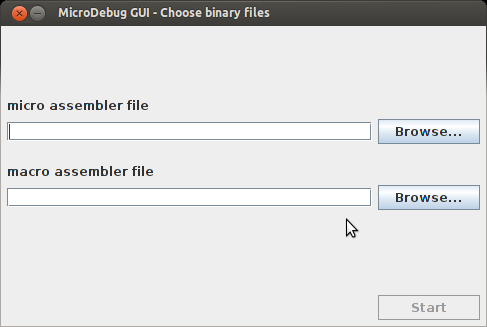
\includegraphics[width=6cm]{images/start-frame-empty}
	\caption{Screenshot des Start-Fensters}
	\label{fig:start-frame-empty}
\end{figure}

Hast Du zwei Pfade eingegeben, wird der Debugger über den Start-Button gestartet. In diesem Moment werden die beiden Bytecode-Dateien auf ihre Gültigkeit geprüft; zuerst die Mikro-Assembler-Datei und dann die Assembler-Datei. Falls eine der Dateien ungültig ist, wird statt dem Debugger erneut das Start-Fenster gezeigt. In diesem Fall ist dann das Textfeld mit der falschen Datei leer, wie beispielsweise in Abbildung \ref{fig:start-frame-both-wrong} zu sehen.

\begin{figure}[h]
	\centering
	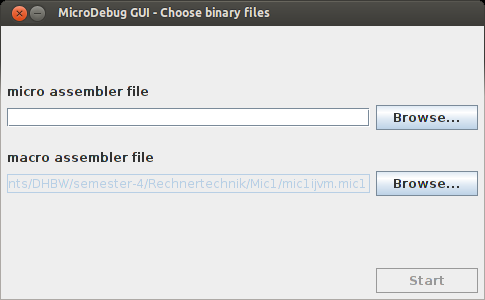
\includegraphics[width=6cm]{images/start-frame-both-wrong}
	\caption{Screenshot des Start-Fensters -- die angegebenen Dateien waren \emph{beide} ungültig}
	\label{fig:start-frame-both-wrong}
\end{figure}

In diesem Beispiel waren beide Dateien falsch, aber nur ein Textfeld ist leer. Die \mdg{} prüft die Dateien nacheinander, ist bereits die erste Datei ungültig, wird die zweite nicht geprüft und zunächst als gültig angenommen. Das Textfeld der zweiten Datei ist nun ausgegraut, Du kannst es aber mit einem Doppelklick wieder editierbar machen. In dem genannten Beispiel habe ich das getan und nun zwei korrekte Dateien eingetragen, wie Du in Abbildung \ref{fig:start-frame-both-filled} sehen kannst.

\begin{figure}[h]
	\centering
	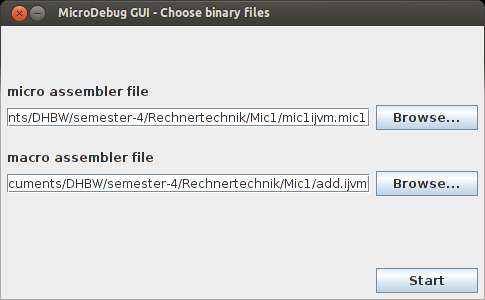
\includegraphics[width=6cm]{images/start-frame-both-filled}
	\caption{Screenshot des Start-Fensters mit zwei eingetragenen Dateien}
	\label{fig:start-frame-both-filled}
\end{figure}

Hast Du dann zwei korrekte Dateien eingetragen, startet der Debugger und du siehst das Hauptfenster aus Abbildung \ref{fig:main-frame-onbegin}.

\begin{figure}[h]
	\centering
	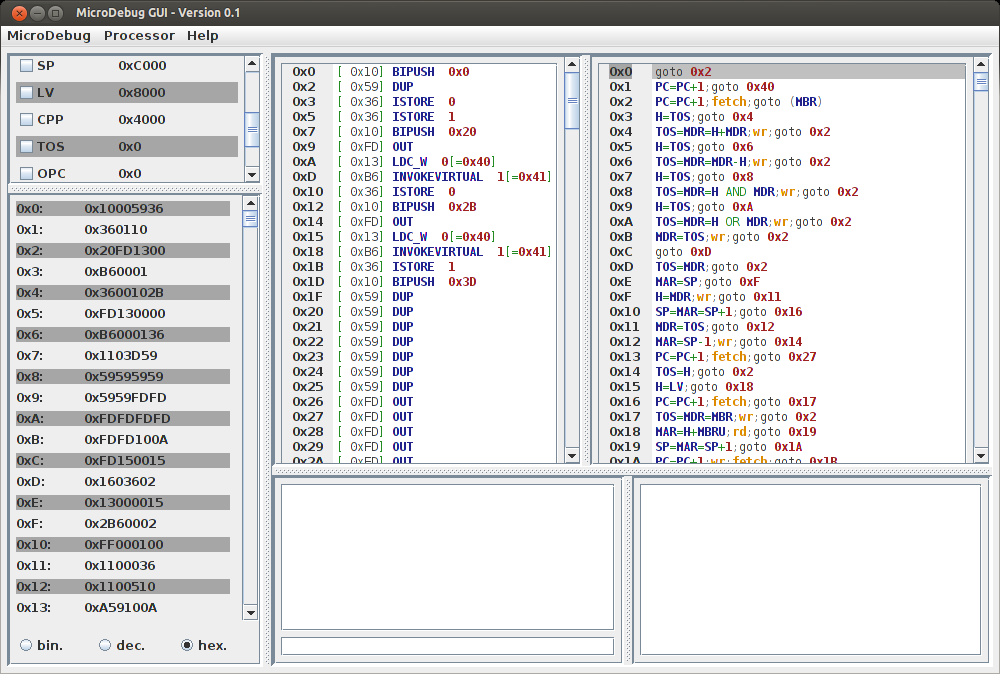
\includegraphics[width=0.8\linewidth]{images/main-frame-onbegin}
	\caption{Hauptfenster der \mdg{} zu Beginn}
	\label{fig:main-frame-onbegin}
\end{figure}

\subsection{Register}
In Abbildung \ref{fig:main-frame-onbegin} siehst Du links oben die Register mit ihren Werten, die gleiche Ansicht ist in Abbildung \ref{fig:main-frame-registers} nochmal größer dargestellt.

\begin{figure}[h]
	\centering
	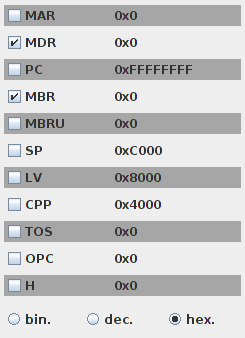
\includegraphics[width=4cm]{images/main-frame-registers}
	\caption{Registeransicht im Hauptfenster der \mdg{}}
	\label{fig:main-frame-registers}
\end{figure}

Die Checkboxen visualisieren die Breakpoints für die Register, in Abbildung \ref{fig:main-frame-registers} hält der Debugger demnach an, wenn \reg{MBR} oder \reg{MDR} im nächsten Zyklus geschrieben wird. Über die Radiobuttons unten kannst Du die Darstellung der Werte ändern, auf binär, dezimal oder hexadezimal -- so kannst Du für jeden Zweck die optimale Darstellung wählen.

\subsection{Hauptspeicher}
Unter der Registeransicht befindet sich im Hauptfenster die Ansicht des Hauptspeichers. Hier kannst du wie bei der Registeransicht die Darstellung der Hauptspeicherwerte jederzeit ändern.

In der Ansicht des Hauptspeichers sind nur eine feste Anzahl an Einträgen zu sehen, die sich nicht dynamisch an die Größe des sichtbaren Bereichs anpassen. Dies habe ich wegen der besseren Performanz so gelöst.

Die Ansicht zeigt den gesamten Hauptspeicher -- neben den lokalen Variablen, dem Stack und den Konstanten kannst Du auch den disassemblierten Assembler-Code in Bit-Form betrachten.

\subsection{Text-Ein- und -Ausgabe}
Rechts neben der Hauptspeicheransicht sind unten verschiedene Textareas zu sehen. Deren Funktion sollte dir spätestens im laufenden Betrieb des Debuggers deutlich werden: Links unten ist das Textfeld, um der \mic{} Text bereitzustellen, darüber befindet sich die Ausgabe der \mic{} und im rechten Bereich tauchen Informationen des \md{} auf, die auf der Konsole sichtbar waren und bisher noch keinen Platz in der Oberfläche bekommen haben.

\begin{figure}[h]
	\centering
	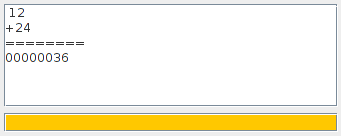
\includegraphics[width=4cm]{images/main-frame-mic-ta}
	\caption{Hauptspeicheransicht im Hauptfenster der \mdg{}}
	\label{fig:main-frame-mic-ta}
\end{figure}

Abbildung \ref{fig:main-frame-mic-ta} zeigt, wie sich das Eingabefeld verhält, wenn die \mic{} per \texttt{IN} ein Zeichen liest, aber der Puffer des \md{} keine Zeichen mehr enthält: es färbt sich orange. In diesem Fall solltest Du die nächste Eingabe eingeben und mit \emph{ENTER} bestätigen. Dadurch werden die eingegebenen Zeichen inklusive Zeilenumbruch im \md{} gepuffert, bis die \mic{} sie einliest.

Du kannst auch Eingaben machen, wenn der Puffer noch nicht leer ist, in diesem Fall wird der Text den du eingibst einfach dem Puffer des \md{} angehängt. So kannst Du schon beim Start des Programms bequem alle nötigen Eingaben machen und die \mdg{} die Eingaben abarbeiten lassen.

\subsection{Code}
Die wichtigsten zwei Komponenten befinden sich in Abbildung \ref{fig:main-frame-onbegin} rechts oben: Der disassemblierte Assembler- und Mikro-Assembler-Code. Die beiden Ansichten sind von der Funktion identisch aufgebaut und zeigen den disassemblierten Code mit Syntaxhervorhebung, Zeilennummern und den dazugehörigen Breakpoints an. Zusätzlich wird die Zeile des Codes hervorgehoben, die als nächstes ausgeführt wird.

\begin{figure}[h]
	\centering
	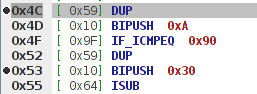
\includegraphics[width=4cm]{images/main-frame-code-part}
	\caption{Ausschnitt der Assembler-Code-Ansicht im Hauptfenster der \mdg{}}
	\label{fig:main-frame-code-part}
\end{figure}

Abbildung \ref{fig:main-frame-code-part} zeigt einen Ausschnitt der Code-Ansicht. Hier kannst Du sehen, dass als nächstes die Zeile \texttt{0x4C} abgearbeitet wird und dass in den Zeilen \texttt{0x4C} und \texttt{0x53} Breakpoints gesetzt sind. Die Breakpoints setzt und entfernst Du durch einen Doppelklick an die Stelle, an der sie gezeichnet werden -- links neben den Zeilennummern.


\section{Tutorial}
\clearpage
        \part{Implementierung}
\chapter{Werkzeuge}
\chplbl{werkzeuge}
In diesem Teil der Arbeit möchte ich besonders eine Frage beantworten: Wie sind die bisher vorgestellten Funktionen des Debuggers implementiert? Mein Ziel ist, die Implementierung und Struktur des Debuggers so nachvollziehbar zu beschreiben, dass Leser mit Programmiererfahrung in der Lage sind, den Debugger weiterzuentwickeln.

Der Debugger soll auch nach Ende dieser Arbeit weiterentwickelt werden können. Daher stelle ich in diesem Kapitel vor, welche Werkzeuge ich zur Entwicklung des Debuggers nutze und wie diese zur Mitarbeit genutzt werden können. Dies ist nicht als Bedienungsanleitung zu verstehen! Ich bin aber der Ansicht, dass es das Verständnis für die Implementierung und meine Arbeit steigert, wenn geklärt ist, welche Werkzeuge ich wie nutze.

\section{Versionskontrollsystem}
Die Projekte \md und \mdg sind bei \name{GitHub} (siehe \cite{Roesch2012,Roesch2012gui}) gehostet und sind somit mit \gls{git} versioniert.

\gls{git} wird beispielsweise in \cite{Ohne1} beschrieben und ist demnach:
\begin{description}
\item[effizient] Auch bei großen Projekten zeigen Vergleiche, dass \gls{git} insgesamt schneller ist, als beispielsweise \gls{svn}.
\item[verteilt] Jeder Entwickler erhält ein lokales Repository und kann damit arbeiten. Es wird kein zentraler Server benötigt, alle Funktionen des Systems und alle Versionen stehen lokal zur Verfügung.
\item[sicher] Bei \gls{git} wird jeder Commit gehasht. Es ist praktisch nicht möglich einen Commit zu manipulieren, da dies die Hash-Summe verändern würde. Auch wenn theoretisch Kollisionen der Hash-Summe möglich sind, ist bisher eine solche Kollision noch nicht konstruierbar -- bei einem Code-Projekt müsste eine solche Kollision zudem kompilierbarer Code sein, was als hinreichend unwahrscheinlich gilt.
\end{description}

Ich habe \gls{git} gewählt, da dadurch später leicht \emph{forks}\footnote{Zu deutsch Abspaltung, ist ein Entwicklungszweig, nachdem sich ein Software-Projekt in zwei oder mehr Teile geteilt hat. Diese Teile werden meist unabhängig voneinander weiterentwickelt. Im täglichen Arbeitsablauf mit \gls{git} ist ein fork aber auch die Möglichkeit Neuerungen für ein Projekt zu Entwickeln und den entstandenen Entwicklungszeig nach Fertigstellung der Neuerung in das Ursprungsprojekt einzupflegen.} gebildet werden können und der Debugger durch Außenstehende weiterentwickelt werden kann. Das dezentrale Entwickeln mit \gls{git} ermöglicht es zusätzlich, dass später viele Entwickler am Debugger mitentwickeln.

Wie checkt man mit \gls{git} den Quelltext der Arbeit aus? Wie unterstützt mich \gls{git}, wenn ich das Projekt weiterentwickeln möchte? Im Folgenden möchte ich auf diese Fragen antworten. Ich möchte keine umfassende Bedienungsanleitung für \gls{git} geben, sondern die Grundlagen für die alltägliche Arbeit mit \gls{git} vermitteln. \gls{git} am \md erklären, für \mdg ist das Vorgehen analog, in den meisten Fällen muss lediglich ein \texttt{-gui} eingefügt werden.

\subsection{Repository klonen und Code auschecken}
\seclbl{git-checkout}
Die Adresse des öffentlichen Repositorys lautet: \code{https://github.com/croesch/micro-debug.git}

\begin{lstlisting}[language=sh,caption={\md mit git klonen},label=\lstlbl{git-klonen}]
git clone git://github.com/croesch/micro-debug.git
cd micro-debug(*@\srclbl{git-klonen-cd}@*)
\end{lstlisting}

Da \gls{git} ein verteiltes Versionskontrollsystem ist, muss das entfernte Repository zunächst lokal angelegt werden -- das wird klonen genannt. Auschecken bezeichnet den Vorgang, den Inhalt aus dem lokalen Repository im Arbeitsverzeichnis zu realisieren, wo er bearbeitet werden kann.

Klont man ein entferntes Repository, beispielsweise das Repository des \md, wird im aktuellen Verzeichnis ein Verzeichnis \texttt{micro-debug} angelegt. In diesem Verzeichnis wird standardmäßig die Kopie des entfernten Repositorys abgelegt -- im Verzeichnis \texttt{micro-debug/.git}. Außerdem wird der Inhalt des Repositorys ausgecheckt und befindet sich anschließend im Verzeichnis \texttt{micro-debug}. \lstref{git-klonen} zeigt, welcher Befehl zum Klonen (und implizit Auschecken) des \md-Repositorys verwendet wird -- in \srcref{git-klonen-cd} wird in das erzeugte Verzeichnis gewechselt, das Arbeitsverzeichnis.

Im Gegensatz zu \gls{svn} erstellt \gls{git} nur im Wurzelverzeichnis eines Projekts ein Verzeichnis \texttt{.git}. Direkt nach dem Klonen eines anderen Repositorys enthält es beispielsweise einen Verweis (\emph{origin}) auf dieses Repository. Sobald das geklonte Repository neuere Commits enthält, kann dieser Verweis genutzt werden, um wie in \lstref{git-pull} die neuen Commits in das lokale Repository zu übernehmen.

\begin{lstlisting}[language=sh,caption={Mit git \emph{pull} auf Originalrepository ausführen},label=\lstlbl{git-pull}]
git pull origin
\end{lstlisting}

Mit dem Befehl \texttt{pull} werden die neuen Commits heruntergeladen, in das lokale Repository übernommen und ausgecheckt.

Dieses Vorgehen ist aufgrund der Änderung des aktuellen Arbeitsverzeichnisses häufig unerwünscht, daher kann man den Befehl aus \lstref{git-pull} wie in \lstref{git-fetch-merge} in zwei Befehle aufteilen, um zu regeln, ob und welcher Branch die Neuerungen erhält.

\begin{lstlisting}[language=sh,caption={\emph{pull} in zwei Befehlen manuell ausführen},label=\lstlbl{git-fetch-merge}]
git fetch origin(*@\srclbl{git-fetch-fetch}@*)
git merge origin/master(*@\srclbl{git-fetch-merge}@*)
\end{lstlisting}

Mit \emph{fetch} in \srcref{git-fetch-fetch} werden die Aktualisierungen heruntergeladen und zunächst im lokalen Repository gespeichert. Erst der Befehl \emph{merge} in \srcref{git-fetch-merge} verändert die Dateien im Arbeitsverzeichnis.

Es gibt bei \gls{git} auch einen expliziten \texttt{checkout}-Befehl, der verwendet wird, um beispielsweise zwischen verschiedenen Branches zu wechseln.

\subsection{Code beitragen}
Hat man ein Repository geklont und möchte Codeänderungen dem Originalrepository zuführen, gibt es zwei Möglichkeiten: Man benutzt den Standard-Branch oder so genannte Feature-Branches.

\begin{lstlisting}[language=sh,caption={Eine Datei mit git committen},label=\lstlbl{git-commit}]
git add relativer-pfad-zur-datei
git commit -m "Commit-Nachricht"
\end{lstlisting}

Den Standard-Branch (\texttt{master}) zu nutzen, empfehle ich nur, wenn man alleine an einem Projekt entwickelt. \lstref{git-commit} zeigt die Befehle, um eine veränderte Datei zu commiten. Dieser Commit wirkt sich auf den aktuellen Branch aus und kann mit dem \texttt{push}-Befehl in das geklonte Repository transferiert werden. Das entfernte Repository muss dazu den gleichen Stand haben, wie das lokale Repository ohne den zu veröffentlichenden Commit.

Da dies insbesondere bei mehrköpfigen Entwicklungsteams eine Herausforderung ist, empfehle ich Feature-Branches zu nutzen. Durch folgende Schritte kann jeder Leser selbst Code zum \md beitragen und diesen veröffentlichen.
\begin{enumerate}
\item Unter \code{https://github.com/croesch/micro-debug/issues} sind die Bugs und offenen Aufgaben zu finden. Möchte jemand Code beitragen, vermerkt er dies an dem jeweiligen Thema, oder öffnet ein neues, falls kein passendes Thema gefunden werden kann.

\item Im lokalen Repository wird nun ein so genannter Feature-Branch angelegt, in dem der Code geändert werden wird. \lstref{git-branch-erstellen} enthält den Befehl, mit dem ein neuer Branch im lokalen Repository angelegt und ausgecheckt wird -- eine Konvention ist, dass die Nummer des Branches der Nummer des Themas entspricht.

\begin{lstlisting}[language=sh,caption={Einen Branch mit git erstellen},label=\lstlbl{git-branch-erstellen}]
git checkout -b 100-themen-titel
\end{lstlisting}

\item Der entsprechende Code kann nun geändert und wie in \lstref{git-commit} committet werden -- die Commits betreffen den neu erstellten Branch.

\item Regelmäßig oder zumindest am Ende der Änderungen sollte der aktuelle Stand des Originalrepositorys geladen werden. Dazu empfehle ich den Branch \texttt{master} auszuchecken und die aktuellen Commits des Originalrepositorys dort einzupflegen -- wie in \lstref{git-master-aktualisieren} zu sehen.

\begin{lstlisting}[language=sh,caption={Mit git den Branch \texttt{master} auschecken und aktualisieren},label=\lstlbl{git-master-aktualisieren}]
git checkout master
git pull origin master
\end{lstlisting}

\item Nun sollte der neu erstellte Branch so verändert werden, dass seine Commits auf dem aktuellen Stand des Repositorys aufsetzen. Dies kann mit dem Befehl \texttt{rebase} erledigt werden, wie in \lstref{git-neubranch-rebase} beschrieben. Das auschecken des neuen Branches ist nötig, da \texttt{rebase} den aktuellen Branch so verändert, dass er auf dem angegebenen Branch aufsetzt; in diesem Fall \texttt{master}.

\begin{lstlisting}[language=sh,caption={Mit git ein \texttt{rebase} auf einen Branch ausführen},label=\lstlbl{git-neubranch-rebase}]
git checkout 100-themen-titel
git rebase master
\end{lstlisting}

\item Zum Schluss ist das lokale Repository in einem Zustand, der veröffentlicht werden kann. \lstref{git-push} zeigt, wie nun der neu erstellte Branch an das Originalrepository gesendet werden kann.
\begin{lstlisting}[language=sh,caption={Mit git einen lokalen Branch an das Originalrepository senden},label=\lstlbl{git-push}]
git push origin 100-themen-titel
\end{lstlisting}
\end{enumerate}

Die Entwickler des Originalrepositorys können den neuen Branch nun einsehen, überprüfen und in den Branch \texttt{master} einpflegen. Dadurch ist er offiziell Teil des Produkts geworden -- diese Vorgehensweise ermöglicht sehr verteiltes Arbeiten bei gleichzeitig zentraler Verwaltung und Entscheidung, welche Änderungen tatsächlich dem Projekt zugeführt werden.

Bei dem Arbeitsfluss, den ich gerade beschrieben habe, ist das lokale Repository ein Klon des Originalrepositorys. In der Regel hat aber nur ein oder wenige Entwickler Schreibrechte auf dem Originalrepository, das alle lesen können. Daher ist in der Praxis noch ein zusätzlicher Schritt nötig, den ich im Folgenden vorstellen möchte.

\subsection{Unterstützung durch GitHub}
Die Idee ist, dass jeder Entwickler sein eigenen öffentlichen Klon des Originalrepositorys besitzt. Dieser öffentliche Klon wird von dem jeweiligen Entwickler lokal geklont, und daran gearbeitet, wie oben beschrieben. Zur Aktualisierung des lokalen Repositorys muss zusätzlich das öffentliche Repository des Entwicklers aktualisiert werden und nach Fertigstellung der Arbeit kann das Ergebnis per \texttt{push}-Befehl in dem Repository des Entwicklers veröffentlicht werden. Der oder die Entwickler des Originalrepository können die veröffentlichten Änderungen dann in das Originalprojekt einfließen lassen.

Für diesen Arbeitsablauf ist \name{GitHub} sehr gut geeignet -- daher möchte ich diesen Arbeitsablauf am Beispiel von \name{GitHub} verdeutlichen.

\begin{enumerate}
\item Bei \name{GitHub} ist eine Registrierung notwendig, um Repositorys veröffentlichen zu können.

\item Ist man nun angemeldet, erscheint auf der Projektseite \cite{Roesch2012} der \emph{fork}-Button. Dadurch klont \name{GitHub} das Projekt für den Benutzer, wo es nun unter \code{https://github.com/benutzername/micro-debug} öffentlich verfügbar ist.

\item Anschließend kann wie in \lstref{git-benutzer-klonen} das öffentliche Repository geklont werden. Der Unterschied zu \lstref{git-klonen} ist die Adresse des geklonten Repositorys und das Protokoll -- das \gls{git}-Protokoll erlaubt Schreib- und Leseoperationen, bei entsprechenden Rechten auf dem Server.

\begin{lstlisting}[language=sh,caption={\md mit git vom Benutzerrepository klonen},label=\lstlbl{git-benutzer-klonen}]
git clone git://github.com/ihr-name/micro-debug.git
cd micro-debug
\end{lstlisting}

\item Um später Aktualisierungen des Originalrepository zu erhalten, sollte dieses noch im lokalen Repository als \texttt{remote} hinzugefügt werden, wie in \lstref{git-add-original-remote} zu sehen.

\begin{lstlisting}[language=sh,caption={Originalrepository des \md dem lokalen Repository als \texttt{remote} hinzufügen},label=\lstlbl{git-add-original-remote}]
git remote add original-projekt git://github.com/croesch/micro-debug.git
\end{lstlisting}

\item Im lokalen Repository wird nun ein Feature-Branch angelegt, wie in \lstref{git-branch-erstellen} beschrieben.

\item Der entsprechende Code kann nun geändert und wie in \lstref{git-commit} committet werden -- die Commits betreffen den neu erstellten Branch.

\item Da sich das öffentliche Repository des Benutzers nicht ändert, können Aktualisierungen nicht wie in \lstref{git-master-aktualisieren} beschrieben in das lokale Repository geholt werden. Daher benötigt das lokale Repository die Referenz auf das Originalrepository, wie in \lstref{git-add-original-remote} erstellt.

\begin{lstlisting}[language=sh,caption={Mit git den Branch \texttt{master} auschecken und aktualisieren},label=\lstlbl{git-master-original-aktualisieren}]
git checkout master
git pull original-projekt master
\end{lstlisting}

\lstref{git-master-original-aktualisieren} enthält die Befehle, um das lokale Repository mit den Informationen aus dem Originalrepository zu aktualisieren.

\item Abschließend sollte der neue Branch wie in \lstref{git-neubranch-rebase} beschrieben neu auf den \texttt{master}-Branch aufgesetzt werden und dann wie in \lstref{git-push} gezeigt, in dem öffentlichen Repository des Benutzers veröffentlicht werden.

\item \name{GitHub} bietet nun die Möglichkeit die Entwickler des Originalprojekts über den neuen Branch im öffentlichen Repository des Entwickelrs zu informieren. Dazu befindet sich auf der Projektseite des Benutzers ein Button \emph{Pull-Request}. Wenn die Entwickler des Originalrepositorys entscheiden die Änderungen in das Projekt aufzunehmen, sind diese Informationen später über die in \lstref{git-master-original-aktualisieren} beschriebene Aktualisierung im Branch \texttt{master} zu sehen.
\end{enumerate}

Meine Ausführungen über \gls{git} sollten es ermöglichen, den Code des \md auszuchecken, zu ändern und die Änderungen zu veröffentlichen. Im Folgenden möchte ich nun das Build-Management-Werkzeug erläutern, dass ich zum Entwickeln nutze: \gls{mvn}.

\section{Build-Management}
\gls{mvn} ist ein Werkzeug zum Bauen von \gls{java}-Anwendungen. Meines Erachtens gibt es keine signifikanten Gründe für oder gegen die Nutzung von \gls{mvn}; stattdessen hätte ich auch \gls{ant} oder \gls{make} nutzen können.

In diesem Abschnitt möchte ich die grundlegenden Befehle für die Arbeit mit \gls{mvn} erläutern.

Ich verwende \gls{mvn}, da hier viel implizites Wissen eingesetzt wird; dadurch wird der Konfigurationsaufwand geringer -- solange man den Konventionen der \gls{mvn}-Entwickler folgt. Zu dem impliziten Wissen gehört unter anderem:
\begin{itemize}
\item \gls{java}-Klassen befinden sich in \code{src/main/java/}
\item \gls{java} Test-Klassen befinden sich in \code{src/test/java/}
\item Ressourcen befinden sich in \code{src/main/resources/}
\item Ressourcen, die nur für die Tests benötigt werden, befinden sich in \code{src/test/resources/}
\item Kompilate und von \gls{mvn} generierte Klassen befinden sich in \code{target/}
\item Die explizite Konfiguration steht in der Datei \code{pom.xml}
\end{itemize}

Die Datei \texttt{pom.xml} enthält aus \gls{mvn}-Sicht alle nötigen Informationen über das Projekt: Die Version, der Name und benötigte Bibliotheken sind einige dieser Informationen.

Das wohl Wichtigste an einer Build-Management-Software ist, den Code kompilieren zu können. \lstref{maven-compile} zeigt den Befehl, mit dem der Code eines \gls{mvn}-Projekts wie dem \md kompiliert werden kann. Testklassen werden dadurch nicht kompiliert und auch nicht ausgeführt.

\begin{lstlisting}[language=sh,caption={Den Code eines Maven-Projekts kompilieren},label=\lstlbl{maven-compile}]
mvn compile
\end{lstlisting}

\gls{mvn} liest die Abhängigkeiten für ein Projekt aus der \texttt{pom.xml} Datei und lädt die benötigten Bibliotheken selbstständig herunter. Auch für die Ausführung von \gls{mvn} werden gewisse Bibliotheken, dies führt bei der ersten Ausführung von \gls{mvn} dazu, dass zunächst einige Bibliotheken heruntergeladen werden.

Bei der Ausführung von \gls{mvn} gibt es verschiedene Ziele, die aufeinander aufbauen. So ist beispielsweise für das Packetieren eines Projekts notwendig zunächst alle Klassen zu kompilieren und die Tests auszuführen, bevor das Projekt packetiert wird. Das Projekt wird mit dem Befehl aus \lstref{maven-package} packetiert und im Verzeichnis \texttt{target/} abgelegt.

\begin{lstlisting}[language=sh,caption={Den Code eines Maven-Projekts packetieren},label=\lstlbl{maven-package}]
mvn package
\end{lstlisting}

Wenn man Änderungen am Code vornimmt, ist es besonders hilfreich zu wissen, ob die automatisierten Tests fehlschlagen. Möchte man mit \gls{mvn} die Tests ausführen, kann dazu der in \lstref{maven-test} gezeigte Befehl genutzt werden.

\begin{lstlisting}[language=sh,caption={Die automatisierten Tests eines Maven-Projekts ausführen},label=\lstlbl{maven-test}]
mvn test
\end{lstlisting}

Die in der Datei \code{pom.xml} definierten abhängigen Projekte sind in \gls{xml} definiert, wie beispielsweise in \lstref{maven-dependency} am Beispiel von \gls{fest} zu sehen, das vom Debugger genutzte \gls{gui}-Test-Framework.

\begin{lstlisting}[language=sh,caption={Konfiguration eines abhängigen Projekts in Maven},label=\lstlbl{maven-dependency}]
<dependency>
    <groupId>org.easytesting</groupId>
    <artifactId>fest-swing</artifactId>
    <version>1.2.1</version>(*@\srclbl{maven-dependency-version}@*)
    <scope>test</scope>
</dependency>
\end{lstlisting}

Dort kann nun die Version von \gls{fest} geändert werden, die der Debugger nutzen soll.

Die hier gezeigten Befehle sind keine umfassende Beschreibung von \gls{mvn}, genügen aber, um den Debugger zu bauen. Für das Kompilieren können auch andere Werkzeuge verwendet werden, allerdings muss der Entwickler sich dann um die Bibliotheken selbst kümmern. Aber prinzipiell ist \gls{mvn} durch jedes beliebige andere Werkzeug ersetzbar.
\chapter{Implementierung der \mic}
\chplbl{prozessor}
Nachdem ich nun die Vorteile der automatisierten Tests genannt habe, möchte ich den Code fokussieren. Ich werde kann hier aus Zeit- und Platzgründen nur gewisse Eckpunkte der Implementierung beleuchten, die verschiedenen Klassen und Methoden sind jeweils gut dokumentiert und sollten nach dem Lesen der folgenden Kapitel schnell verstanden werden können.

Der erste Schritt bei der Implementierung des Debuggers ist die Simulation der \mic, erst wenn dies zufriedenstellend funktioniert, können die Debug-Funktionen entwickelt werden. Ich möchte daher in diesem Kapitel die Implementierung des Prozessors anschauen und zeigen, welche Besonderheiten es gibt.

Für die Implementierung der \mic ist es nötig, sich ein Abstraktionsniveau auszusuchen, auf dem implementiert wird. In den folgenden Abschnitten ist zu sehen, dass ich mich für eine relativ hardwarenahe Implementierung entschieden habe. Daher habe ich zunächst folgende zu implementierende Komponenten identifiziert: die \gls{alu} inklusive Shifter, die Register, den Mikro-Code-Speicher inklusive der darin abgelegten Instruktionen und der Hauptspeicher.

Aufgrund der \gls{mvn}-Architektur liegt der \gls{java}-Code in dem Verzeichnis \texttt{src/main/java/} und die entsprechenden Tests dazu in \texttt{src/test/java/}. In diesen Verzeichnissen ist eine \package-Struktur erkennbar, die unter dem \package \pck{com.github.croesch.micro_debug} beginnt, alle Klassen des Debuggers sind in diesem \package oder in \subpackages zu finden.

Auch der Code für die \mic befindet sich in einem solchen \subpackage: \pck{com.github.croesch.micro_debug.mic1}. In diesem Verzeichnis gibt es die Klasse \klasse{Mic1}, die ich in \secref{mic-zusammensetzung} genauer beschreiben werde. Alle weiteren Klassen, die den \mic bilden sind in folgenden \subpackages zu finden:
\begin{description}
\item[alu] bildet die \gls{alu} ab und ist in \secref{mic-alu} beschrieben.
\item[api] enthält einige Interfaces, um die Implementierung der \mic unabhängig gestalten zu können.
\item[controlstore] bildet den \mac-Speicher und die \mais ab und ist in \secref{mic-instructions} beschrieben.
\item[io] bildet die Ein- und Ausgabe der \mic ab. Die Klasse \klasse{Input} dient zum Einlesen einzelner Zeichen und enthält einen Puffer, der die noch nicht von der \mic gelesenen Zeichen enthält, da vom Benutzer nur zeilenweise Eingaben gemacht werden können.

Die Klasse \klasse{Output} dient zur Ausgabe einzelner Zeichen und puffert, falls die Ausgabe gepuffert erfolgen soll, die ausgegebenen Zeichen bis ein Zeilenumbruch ausgegeben wird.
\item[mem] bildet den Hauptspeicher ab und ist in \secref{mic-mem} beschrieben.
\item[mpc] bildet die Komponenten ab, die zusammen für die Berechnung des nächsten \gls{mpc} verantwortlich sind und ist in \secref{mic-mpc} beschrieben.
\item[register] bildet die Register der \mic ab und ist in \secref{mic-register} beschrieben.
\item[shifter] bildet den Shifter ab und ist in \secref{mic-alu} beschrieben.
\end{description}

Die \package-Struktur sollte bereits einen groben Überblick geben, wo welche Komponenten implementiert sind. Zum besseren Verständnis möchte ich nun nochmal die Hardware-Komponenten der \mic betrachten und ihre Implementierungen beschreiben.

\section{ALU}
\seclbl{mic-alu}
Die \gls{alu} der \mic setzt sich aus 32~Ein-Bit-\gls{alu}s zusammen -- so ist die \gls{alu} auch implementiert. Die Klasse \klasse{Alu} benutzt 32~Instanzen der Klasse \klasse{OneBitAlu}, zur Berechnung der Ausgabewerte -- damit ist die \gls{alu} die Komponente, die am hardwarenahesten implementiert ist.

Die Klasse besitzt eine Methode \texttt{calculate()}, in der aus den Eingangssignalen das Ausgangssignal der \gls{alu} berechnet wird; dieses Signal wird an den Shifter weitergeleitet. Die Klasse \klasse{Shifter} im gleichnamigen \package bildet den Shifter ab und besitzt ebenso eine Methode \texttt{calculate()}, um die Verarbeitung der Signale anzustoßen.

Die Berechnung der \gls{alu} und des Shifters werden bei jedem Zyklus der \mic angestoßen. Durch die sehr hardwarenahe Implementierung bilden sie daher vermutlich ein Performance-Engpass zur Laufzeit des \md.

\section{Register}
\seclbl{mic-register}
Die Dateneingänge der \gls{alu} werden mit den Inhalten zweier Register gefüllt und das Ergebnis des Shifters wird wiederum in verschiedene Register geschrieben. Die Register sind im \md als Enumeration \klasse{Register} im gleichnamigen \package implementiert. Sie erfüllen lediglich die Aufgabe einer 32~Bit Variable.

Das Register \reg{MBR} kann im \mic mit oder ohne Vorzeichenerweiterung gelesen werden. Dieses Verhalten ist im \md dadurch realisiert, dass es ein Register \reg{MBR} und ein Register \reg{MBRU} gibt. \reg{MBRU} enthält den Wert ohne Vorzeichenerweiterung und das Register \reg{MBR} enthält den Wert mit Vorzeichenerweiterung. Bei der Vorzeichenerweiterung wird wie bei der \mic davon ausgegangen, dass der ursprüngliche Wert in 8~Bit vorlag.

Dass die Register als Enumeration implementiert sind hat den Vorteil, dass man von allen Klassen leicht auf die Register zugreifen kann, aber den Nachteil, dass allein durch die Code-Struktur nicht deutlich wird, zu welcher logischen Einheit die Register gehören.

\section{Mic1-Instruktionen}
\seclbl{mic-instructions}
Welche Berechnung mit welchen Registerwerten ausgeführt wird und in welches Register das Ergebnis geschrieben wird, regeln die Signale der \mais. Die \mais (\klasse{MicroInstruction}) sind im \mac-Speicher (\klasse{MicroControlStore}) abgelegt.

Zur besseren Lesbarkeit des Codes nutzt die Implementierung der \mai Unterklassen von \klasse{SignalSet}, um die verschiedenen Signale zu gruppieren. Die Darstellung der \mai für den Benutzer ist in der Klasse \klasse{MicroInstructionDecoder} implementiert. Wie wird eine \mai erzeugt? Der \mac-Speicher ist in der \datei{mic1} definiert; aus dieser Datei kann die Klasse \klasse{MicroInstructionReader} einzelne \mais erzeugen.

Meine Implementierung der \mai, der Darstellung einer \mai und dem Einlesen einer \mai basieren auf der Implementierung von \name{Ontko}. \name{Ontko} hat in \cite{Ontko1999} einen Simulator für die \mic in \gls{java} entwickelt, der bereits Komponenten zur Darstellung und zum Einlesen von \mais implementiert hat.

\section{MPC-Berechnung}
\seclbl{mic-mpc}
Der \gls{mpc} bestimmt, welche \mai im nächsten Zyklus ausgeführt werden soll. In der \mic sind mehrere Komponenten gemeinsam für die Berechnung des \gls{mpc} verantwortlich. Diese verschiedenen Komponenten habe ich in der Klasse \klasse{NextMPCCalculator} zusammengefügt; auch hier gibt es eine Methode \texttt{calculate()} zum Verarbeiten der Eingangssignale.

\section{Hauptspeicher}
\seclbl{mic-mem}
Der Stack, der \ac und die Konstanten liegen im Hauptspeicher; mit diesem kommuniziert die \mic über die Register \reg{MAR}, \reg{MDR}, \reg{MBR} und \reg{PC}. Der Hauptspeicher ist in der Klasse \klasse{Memory} implementiert; der Speicher selbst ist in einem \emph{int}-Array abgebildet, weswegen der Hauptspeicher im \md wortweise adressiert wird.

Die \ais im Hauptspeicher sind nicht so sauber implementiert wie die \mais: sie sind im \emph{int}-Array abgelegt. Lediglich für das disassemblieren werden die Zahlenwerte anhand der Datei \texttt{ijvm.conf} durch den \klasse{IJVMConfigReader} in Instruktionsobjekte (\klasse{IJVMCommand} inklusive \klasse{IJVMCommandArgument}) gepackt.

\section{Zusammensetzung der Komponenten}
\seclbl{mic-zusammensetzung}
Die einzelnen Komponenten werden in der Klasse \klasse{Mic1} zusammengeführt und nach außen als ein Prozessor dargestellt. Lediglich für gewisse Debug-Funktionen ist der Zugriff auf einzelne Komponenten, wie beispielsweise die Register, zugelassen.

Die Klasse \klasse{Mic1} bekommt im Konstruktor zwei Objekte der Klasse \klasse{InputStream} -- eines enthält den \ma und das andere den \ac. Mit diesen beiden Objekten wird dann der \mac-Speicher und der Hauptspeicher erzeugt, die jeweils selbst für das Lesen des Bytecodes verantwortlich sind. Stimmt eine \emph{magic number} nicht, oder sind die Eingabedateien aus anderen Gründen ungültig, wird eine \emph{Exception} geworfen.

Auf die einzelnen Methoden möchte ich hier nicht eingehen, bis auf eine: In der Methode \texttt{doTick()} wird ein einzelner Zyklus der \mic ausgeführt. Diese Methode ist nur für Testzwecke sichtbar und wird von außen über die Methoden \texttt{run()}, \texttt{step()} und \texttt{microStep()} aufgerufen, die unterschiedlich viele Zyklen auf einmal abarbeiten lassen.

Aufgrund der gesammelten Funktionalität ist die Klasse \klasse{Mic1} eine der größten und damit komplexesten im \md.
\chapter{Implementierung der Konsolenvariante}
\chplbl{konsole}
Das Verständnis über die Simulation der \mic haben wir nun erlangt und wollen uns jetzt dem \md selbst widmen. In den folgenden Abschnitten möchte ich in \secref{k-ablauf} zunächst skizzieren, welche Klassen im Programmablauf welche Rolle spielen. Danach möchte ich in \secref{k-konfiguration} erläutern, wie die Konfigurationsdateien gelesen werden und in \secref{k-lokalisierung} wie die Lokalisierungsdateien interpretiert werden. Am Ende dieses Kapitels möchte ich in \secref{k-packages} die einzelnen \packages{} beschreiben, damit du einen vollständigen Überblick über den Code des \md erhälst.

\section{Programmablauf}
\seclbl{k-ablauf}
Nachdem Du den \md das ein oder andere Mal benutzt hast, ist wahrscheinlich der einfachste Einstieg in den Code am Programmablauf zu erklären. Daher möchte ich in diesem Abschnitt einige Schritte im Programmablauf aufgreifen und die beteiligten Klassen erwähnen.

\subsection{Verarbeitung der Argumente}
Wie Du an den Startskripten erkennen kannst ist die \texttt{main()}-Methode in der Klasse \klasse{MicroDebug} enthalten. In dieser Klasse wird zunächst geprüft, wie viele Argumente der Benutzer angegeben hat und dann entsprechende Aktionen eingeleitet.

Wir nehmen nun an, der Benutzer möchte den \md starten und hat daher mindestens zwei Argumente angegeben; in diesem Fall verarbeitet die Methode \texttt{createArgumentList(String[])} in der Klasse \klasse{AArgument} die Argumente. Diese Klasse ist auch gleichzeitig die Basisklasse für alle verfügbaren Argumente. Die Argumente, die jeweils noch Parameter besitzen können, werden dann in der Methode \texttt{executeTheArguments(Map<AArgument, String[]>)} nacheinander ausgeführt.

Hier wird die Methode \texttt{execute(String ...)} an jedem Argument mit den dazugehörigen Parametern ausgeführt. Diese Methode gibt einen Wahrheitswert zurück, der bestimmt, ob der \md nach Ausführung des Arguments starten darf oder nicht.

\subsection{Aufbau der Debugumgebung}
\seclbl{k-aufbau-debugger}
Nachdem die Argumente abgearbeitet wurden und der \md starten darf, werden die beiden Bytecode-Dateipfade eingelesen und in Objekte der Klasse \klasse{InputStream} verwandelt. Dann wird, wie im vorherigen Kapitel beschrieben, mit diesen beiden Objekten die \mic erzeugt. Hierbei kann es sein, dass bereits im Konstruktor eine \emph{Exception} auftritt, wenn eine der Dateien nicht das erwartete Format haben. Daher kümmert sich die Klasse \klasse{MicroDebug} auch um die Fehlerbehandlung.

Ist die \mic erzeugt, kann nun die Umgebung des eigentlichen Debuggers gestartet werden. Hier ist die zentrale Klasse die \klasse{Debugger}: in dieser Klasse befindet sich die Schleife zum Einlesen der Benutzerinstruktionen, aber dazu im \secref{k-benutzerinstruktionen} mehr. In der Klasse \klasse{Debugger} wird auch eine Instanz der Klasse \klasse{Mic1Interpreter} erzeugt, die die eigentlichen Debug-Funktionen sammelt und delegiert. Sie dient besonders als Abstraktionsebene zwischen Benutzerinstruktionen und dem Prozessor \mic, so dass die \mic nicht mit Debug-Funktionalität gefüllt wird.

Die Klasse \klasse{Mic1Interpreter} delegiert einige Funktionalität an zwei wichtige Klassen, die hier erzeugt werden: \klasse{TraceManager}, zum Beobachten von Prozessorvariablen und \klasse{MemoryInterpreter}, der eine Abstraktionsebene über der Klasse \klasse{Memory} darstellt und den Assembler-Code disassemblieren kann.


\subsection{Verarbeitung der Benutzerinstruktionen}
\seclbl{k-benutzerinstruktionen}
Nachdem nun die Argumente verarbeitet wurden, die \mic erzeugt wurde und die Debug-Funktionen initialisiert wurden, wird in der Klasse \klasse{MicroDebug} die Methode \texttt{run()} an der Klasse \texttt{Debugger} aufgerufen und damit die Schleife für die Bearbeitung der Benutzerinstruktionen gestartet. Das Erzeugen der Benutzerinstruktionen funktioniert ähnlich, wie das Erzeugend er Argumente: die Methode \texttt{of(String)} der Klasse \klasse{UserInstruction} wandelt einen \emph{String} in eine Benutzerinstruktion um.

Anschließend wird diese mit den eventuellen Parametern ausgeführt: mit der Methode \texttt{execute(Mic1Interpreter,String ...)}. Der Unterschied zu der Verarbeitung der Argument ist, dass die Benutzerinstruktionen keine Klassenhierarchie bilden, sondern in einer Enumeration implementiert sind. Demzufolge enthält die Klasse \klasse{UserInstruction} die Implementierung aller Benutzerinstruktionen -- was sie zu einer der größten und komplexesten Klassen im \md macht.

Auch diese Methode gibt einen Wahrheitswert zurück -- dieser gibt an, ob der \md nach Ausführung der Benutzerinstruktion beendet werden soll oder nicht. Beendet der Benutzer den Debugger mit dem Befehl \texttt{EXIT}, dann terminiert die Methode \texttt{run()} in \klasse{Debugger} und damit auch am Ende die \texttt{main()}-Methode in \klasse{MicroDebug}.

\subsection{Verarbeitung der Konfiguration}
\seclbl{k-konfiguration}
Der Benutzer hat (wie in \secref{konfiguration} beschrieben) die Möglichkeit, den \md zu konfigurieren. Das Einlesen der Konfiguration geschieht implizit, das heißt wenn die erste Konfigurationsoption benötigt wird.

Das \package{} \pck{settings} enthält verschiedene Klassen, die alle einen anderen Typ von Konfigurationsoption enthalten. Diese Klassen sind als Enumerations implementiert und nutzen meist die Klasse \klasse{PropertiesProvider} -- die Klasse, die Zugriff auf die tatsächlichen Dateien hat. Dieser Mechanismus ist etwas komplex, daher möchte ich hier die einzelnen Schritte erklären, die beim Abfragen der ersten Konfigurationsoption ausgeführt werden:

\begin{enumerate}
\item An der Klasse \klasse{PropertiesProvider} wird die Methode \texttt{getInstance()} aufgerufen und damit die einzige Instanz der Klasse erzeugt.
\item An diesem Objekt wird die Methode \texttt{get(String,String)} aufgerufen, die einen Dateinamen und den Schlüssel der Konfigurationsoption erhält.
\item Das Objekt ruft an sich selbst \texttt{getProperties(String)} mit dem Dateinamen auf.
\item Das Objekt hält eine \emph{Map} mit einem \emph{Properties}-Objekt für jeden Dateinamen, da diese \emph{Map} noch leer ist, wird die Methode \texttt{createNewProperties(String)} mit dem Namen der Datei aufgerufen. Diese Methode wird von jeder Unterklasse überschrieben und liest die Datei nun ein und erzeugt ein \emph{Properties}-Objekt, welches nun in die \emph{Map} gelegt wird, um bei späteren Aufrufen darauf zuzugreifen.\itmlbl{create-props}
\item Dieses \emph{Properties}-Objekt wird nun einige Methodenaufrufe zurückgereicht und daran wird dann die Methode \emph{getProperty(String)} aufgerufen, um den Wert der Konfigurationsoption zu erhalten.
\item Der erhaltene Wert wird nun bis in den Konstruktor der Enumeration zurückgegeben und dort auf Validität überprüft. Stellt sich heraus, dass der Wert ungültig ist, wird die Konfigurationsoption mit einem Standardwert belegt. Das Ergebnis steht dem Benutzer dann zur Verfügung.
\end{enumerate}

Die Klasse \klasse{PropertiesProvider} erbt von \klasse{APropertiesProvider}, die einige der gerade beschriebenen Funktionalität enthält. Es gibt nämlich weitere Unterklassen, die Beispielsweise Konfigurationen aus \datei{xml}en lesen.

\subsection{Verarbeitung der Lokalisierung}
\seclbl{k-lokalisierung}
Die Verarbeitung der Lokalisierung geschieht analog zur im \secref{k-konfiguration} beschriebenen Verarbeitung der Konfiguration.

Allerdings werden die Lokalisierungsdateien aus \datei{xml}en gelesen und deshalb die Klasse \klasse{XMLPropertiesProvider} genutzt. Der einzige Unterschied besteht in \itmref{create-props} des Ablaufs in \secref{k-konfiguration}: Statt einem gewöhnlichen \emph{Properties}-Objekt wird hier ein Objekt der Klasse \klasse{XMLI18nProperties} erzeugt. Diese Klasse ist für das in \secref{lokalisierung} beschriebene Verhalten verantwortlich: Im Konstruktor liest sie die Dateien von allgemein nach spezifisch und ergänzt beschreibt so die erzeugten Key/Value-Paare.

\section{\packages}
\seclbl{k-packages}
Nachdem Du nun die Hauptklassen des \md kennen gelernt hast und nun einen groben Überblick über die Klassen haben solltest, möchte ich nun nochmal alle \packages{} erwähnen und kurz ihren Inhalt beschreiben. Danach solltest Du für die meisten Eigenschaften des \md ein Gefühl haben, wo die Implementierung zu finden ist. Der \md besteht aus folgenden \packages{}:

\begin{description}
\item[annotation] dieses \package{} enthält nur Annotationen. Zur Zeit \texttt{@Nullable} und \texttt{@NotNull}, die dazu genutzt werden, um Methoden zu markieren, ob sie \texttt{null} zurückgeben oder nicht. Auch Variablen können damit markiert werden, um zu definieren, ob sie den Wert \texttt{null} annehmen können oder nicht. Diese Annotationen helfen bei der Navigation durch den Code, denn einmal analysiert und markiert erspart man sich beim nächsten Betrachten der Methode die Analyse.
\item[argument] enthält die Klasse \klasse{AArgument} und ihre Unterklassen -- somit alle möglichen Argumente des \md.
\item[commons] enthält Klassen, die nicht zugeordnet werden konnten. Beispielsweise \klasse{Reader} und \klasse{Printer}, die für die Ein- und Ausgabe des \md verantwortlich sind. Auch die Klasse \klasse{Utils} befindet sich hier -- sie enthält einige Methoden, die keinem genauen Objekt und keiner Klasse zugeordnet werden konnten, wie beispielsweise die Methode \texttt{toBinaryString(int)}, die eine Zahl in eine Zeichenkette wandelt, die die Binärrepresentation der Zahl darstellt.
\item[console] enthält die Debug-Klassen, die speziell für die Benutzung per Konsole konzipiert sind. Hier sind die Klassen \klasse{Debugger}, \klasse{UserInstruction} und \klasse{Mic1Interpreter} zu finden.
\item[debug] enthält Klassen, die mit Breakpoints zu tun haben. Hier sind sowohl der \klasse{BreakpointManager} zu finden, als auch die verschiedenen Unterklassen von \klasse{Breakpoint}, die die verschiedenen Breakpoints darstellen. Diese Unterklassen von \klasse{Breakpoint} müssen nur in dem \package{} sichtbar sein -- für den \klasse{BreakpointManager}.
\item[error] enthält eigene \emph{Exceptions}.
\item[i18n] enthält die Enumeration \klasse{Text}, die die Klasse \klasse{XMLPropertiesProvider} nutzt, um Textkonstanten aus den Lokalisierungsdateien zu lesen und im ganzen Programm verfügbar zu machen.
\item[mic1] wie in \chpref{prozessor} beschrieben.
\item[parser] enthält das Interface \klasse{IParser} und dessen Unterklassen: \klasse{IntegerParser} und \klasse{RegisterParser}, die aus Zeichenketten das entsprechende Objekt parsen. \klasse{IntegerParser} liest beispielsweise Zahlen ein nach dem in \secref{zahlenformat} beschriebenen Zahlenformat und gibt ein \emph{Integer}-Objekt zurück.
\item[properties] enthält die Logik, wie Konfigurationsdateien einzulesen und zu speichern sind. Hier sind beispielsweise die Klassen \klasse{APropertiesProvider}, \klasse{PropertiesProvider}, \klasse{XMLPropertiesProvider} und \klasse{XMLI18nProperties} zu finden.
\item[settings] enthält verschiedene Einstellungs-Enumerationen, zur Zeit eine für intern und eine vom Benutzer zu ändernde. Angedacht ist, dass künftig in der Datei \texttt{micro-debug.properties} nicht nur ganzzahlige Einstellungen stattfinden, sondern auch Wahrheitswerte oder Farbeinstellungen. Jeder Datentyp hätte dann in diesem \package{} eine Klasse, die alle auf die selbe Datei zugreifen. So wäre intern die Typsicherheit gewährleistet und der Benutzer hätte in einer einzigen Datei alle Einstellungen, die er je nach Konfigurationsoption mit Zahlenwerten, Wahrheitswerten oder sonstigem angibt.

Für jeden Datentyp kann hier eine eigene Enumeration genutzt werden, die eine Unterklasse von \klasse{PropertiesProvider} nutzt, da diese Klasse wie in \secref{k-konfiguration} beschrieben die Dateien in einem Zwischenspeicher hält. Dadurch wird jede Konfigurationsdatei nur einmal gelesen und kann dann von den verschiedenen Einstellungs-Enumerationen ausgewertet werden -- jede Enumeration nutzt die Werte aus der Datei, die sie selbst benötigt.
\end{description}

Du hast nun eine Übersicht über den \md und seine Implementierung erhalten. Nochmal wiederholt, die wichtigsten Klassen des \md sind: die Startklasse \klasse{MicroDebug}, die Enumeration der Benutzerinstruktionen \klasse{UserInstruction}, die \mic \klasse{Mic1} und die Schleife zum Einlesen der Benutzerinstruktionen in \klasse{Debugger}.
\chapter{Implementierung der GUI}
\chplbl{gui}
In diesem Kapitel möchte ich vorstellen, wie die \mdg den \md nutzt und welche Klassen hier welche Rolle einnehmen. Ähnlich wie in \chpref{konsole} möchte ich im \secref{gui-ablauf} die Komponenten anhand des Programmablaufs der \mdg vorstellen. In \secref{g-bibliotheken} möchte ich die verwendeten Bibliotheken vorstellen, die der Benutzer am Ende erhält und deren Bedeutung für die \mdg erläutern. Am Ende dieses Kapitels möchte ich auch hier nochmal alle \packages aufführen und beschreiben, welche Funktionalität dahinter steckt und eventuell einzelne Klassen erwähnen.

Die \mdg ist ein eigenständiges Projekt und vom Code her ein Benutzer des \md. Alle Implementierungen der \mdg haben also keinerlei Auswirkung auf den \md, umgekehrt allerdings schon. Wie in \secref{gui-nutzung-konsole} beschrieben ist es daher möglich, dass bei vorliegender \mdg auch der \md eigenständig genutzt werden kann.

Im Unterschied zur Implementierung des \md befinden sich in der \mdg alle Klassen im \package \pck{com.github.croesch.micro_debug.gui} oder in \subpackages davon. Das verhindert, dass gleichnamige \packages oder Klassen zwischen \md und \mdg zu Problemen führen. Außerdem ist je nach Packetierung die Struktur der packetieren \mdg übersichtlicher.

\section{Programmablauf}
\seclbl{gui-ablauf}
Wie in \secref{k-ablauf} möchte ich zunächst den Start der \mdg betrachten und zeigen, welche Klassen an welchen Aktionen beteiligt sind. Gelegentlich werde ich erwähnen, wo Zugriffe auf den \md stattfinden oder wann der Benutzer gefragt ist.

\subsection{Verarbeitung der Argumente}
Analog zum \md gibt es auch in der \mdg eine Klasse \klasse{MicroDebug}, die die \texttt{main()}-Methode enthält. Allerdings ist es hier irrelevant, wie viele Argumente der Benutzer eingegeben hat, oder ob er überhaupt welche eingegeben hat.

Die \mdg nutzt auch den Mechanismus der Klasse \klasse{AArgument}. Da die \mdg allerdings andere Argumente als der \md besitzt, müssen die neuen Argumente zunächst an der Klasse \klasse{AArgument} registriert werden. Die Argumente der \mdg sind im \package \pck{argument} zu finden; registriert werden diese in der Methode \texttt{createListOfPossibleArguments()} der Klasse \klasse{MicroDebug}.

Nachdem die textuellen Argumente in Objekte vom Typ \klasse{AArgument} konvertiert wurden, werden diese ausgeführt und geben auch jeweils einen Wahrheitswert zurück, ob die \mdg starten darf oder nicht.

\subsection{Aufbau der grafischen Oberfläche}
Darf die \mdg starten, so wird eine Instanz der Klasse \klasse{Mic1Starter} erzeugt, die die \mdg starten kann. Zunächst erzeugt die Klasse jedoch das Startfenster aus \figref{start-frame-empty}, welches in der Klasse \klasse{StartFrame} definiert ist, und zeigt dieses an. Das Startfenster enthält einige Aktionsmöglichkeiten -- hat der Benutzer nun die richtigen Dateien ausgewählt und den Button zum Start gedrückt, wird an der Klasse \klasse{Mic1Starter} die Methode \texttt{create(String,String)} mit den zwei angegebenen Dateipfaden ausgeführt.

Wie in \secref{k-aufbau-debugger} wird nun anhand dieser Dateipfade versucht die \mic zu erzeugen. Gelingt dies nicht, wird das Startfenster erneut gezeigt. Hat der Benutzer zwei korrekte Dateien angegeben, wird das Hauptfenster aus \figref{main-frame-onbegin} aufgebaut und angezeigt, was in der Klasse \klasse{MainFrame} definiert ist.

In der Klasse \klasse{MainFrame} werden drei erwähnenswerte Objekte erzeugt: die \emph{View}, der \emph{Controller} und die \emph{Actions}. Die \emph{View} bildet die Oberfläche und ist zunächst in der Klasse \klasse{MainView} definiert, die wiederum weitere Klassen zur Darstellung der einzelnen Bereiche nutzt. Ein ähnliches Konzept nutzt der \emph{Controller}, der in der Klasse \klasse{MainController} definiert ist: Für die einzelnen kleinen \emph{Views} werden entsprechende \emph{Controller} erzeugt, die dadurch jeweils nur einen kleinen Aufgabenbereich erhalten. Das dritte Objekt ist von der Klasse \klasse{ActionProvider} und erzeugt die \emph{Actions}, die der Benutzer über die Oberfläche ausführen kann. Dieser \emph{ActionProvider} hält die Referenzen auf die \emph{Actions}, so dass nur dieses eine Objekt weitergereicht werden muss anstatt dutzender \emph{Actions}.

Diese \emph{Actions} werden dann in der \klasse{MainMenuBar} in Menüeinträgen visualisiert und mit Tastenkombinationen versehen, die der Benutzer konfigurieren kann.

\subsection{Verarbeitung von Benutzeraktionen}
\seclbl{verarbeitung-benutzeraktionen-threads}
Nachdem die Oberfläche aufgebaut ist, sind die \emph{Actions} der Ausgangspunkt von weiteren Code-Ausführungen. Bis der Benutzer die \texttt{EXIT}-Aktion ausführt oder das Fenster schließt, läuft die \mdg.

In der Klasse \klasse{ActionProvider} werden die Referenzen auf die \emph{Actions} gehalten und unter den Schlüsseln abgelegt, die die Enumeration \klasse{Actions} bietet.

Bis auf einige Ausnahmen werden die verschiedenen \emph{Actions} auf dem \gls{edt} ausgeführt. Bei einigen \emph{Actions} wäre dies von Nachteil: spätestens wenn die \mic eine Eingabe erwarten würde, käme es zu einem Deadlock\notiz{Deadlock erklärn!?}. Denn die Eingabe für die \mic wird in der \mdg über ein Textfeld ausgeführt. Liest die \mic nun auf dem \gls{edt} ein Zeichen aus diesem Textfeld, obwohl dort noch keines eingegeben wurde, dann blockiert der aktuelle Thread (in diesem Fall der \gls{edt}) bis der Benutzer eine Eingabe gemacht hat. Eine Eingabe kann aber nur über den \gls{edt} ausgeführt werden, der noch blockiert ist -- ein Deadlock.

Aus diesem Grund gibt es die Klasse \klasse{AbstractExecuteOnWorkerThreadAction}. Jede \emph{Action}, die davon ableitet, wird nicht auf dem \gls{edt} ausgeführt sondern auf einer Instanz der Klasse \klasse{WorkerThread}. Dieser Thread läuft und arbeitet kontinuierlich Objekte der Klasse \klasse{Runnable} ab und wird hier genutzt, um solche Deadlocks zu umgehen.

\subsection{Konfiguration und Lokalisierung}
Das Lesen der Konfiguration und der Textkonstanten funktioniert analog zu den Ausführungen in \secref{k-konfiguration} und \secref{k-lokalisierung}.

Allerdings nutzt die \mdg eigene Enumerations-Klassen: die Klasse \klasse{GuiText} für die Textkonstanten und die Klassen im \package \pck{settings} zum Verarbeiten der Konfiguration. Somit können Komponenten der \mdg sowohl auf die Konfiguration des \md als auch der \mdg zugreifen und auch auf Textkonstanten aus beiden Projekten.

Wie in \secref{lokalisierung} bereits erwähnt, nutzt die \mdg zur Lokalisierung eine eigene Datei-Hierarchie: Alle \datei{xml}en, die mit \texttt{text-gui} beginnen, enthalten Textkonstanten für die \mdg. Bei der Konfiguration wird allerdings die selbe Datei verwendet, die der \md auch nutzt. Das hat für den Benutzer den Vorteil, dass er nur eine Datei zu pflegen hat.

Für die Pflege des Projekts \mdg bedeutet dies aber, dass sowohl die \datei{xml}en, die nur mit \texttt{text} beginnen, als auch die Konfigurationsoptionen des \md in der Datei \texttt{micro-debug.properties} aktualisiert werden müssen, wenn die Version des benutzten \md geändert wird. Denn diese Dateien werden im Verzeichnis \texttt{java/main/ressources/} gepflegt und sind eigenständig, das heißt, sie werden nicht automatisch aktualisiert, wenn sich die entsprechenden Dateien im \md ändern. Da der \md und die \mdg aber derzeit beide zusammen entwickelt werden, ist dies noch kein Problem.

\section{Bibliotheken}
\seclbl{g-bibliotheken}
Wie gerade angemerkt, wird der \md von der \mdg benutzt. Der Code des \md muss also der \mdg vorliegen; derzeit wird der \md der \mdg als \datei{jar} übergeben und dem Klassenpfad hinzugefügt. Dies ermöglicht es dem Benutzer, die verwendete Version des \md auszutauschen.

Die \mdg enthält nur die \gls{gui}, das komplette Wissen über die \mic ist in der Bibliothek -- dem \md -- enthalten. Diese Bibliothek ist also sehr wichtig und in der Regel nicht vorgesehen, um vom Benutzer durch neuere Versionen ersetzt zu werden.

Eine weitere Bibliothek, die der Benutzer erhält, ist das miglayout (siehe dazu ausführlich \cite{Mig2011}). Diese Bibliothek wird benötigt, um die Oberflächenelemente zu positionieren. Das miglayout bietet eine komfortable und mächtige Schnittstelle, um Komponenten zu positionieren.

Die Bibliothek miglayout wird zwar auch zwingend benötigt, kann aber durchaus durch neuere Versionen ersetzt werden. Auch wenn prinzipiell das Risiko der Inkompatibilität zu künftigen Versionen besteht, ist das Risiko hier geringer, da nur sehr wenige Schnittstellen genutzt werden.

An dieser Stelle möchte ich auch das Testframework \gls{fest} erwähnen: Die dazugehörigen Bibliotheken werden zwar nicht an den Benutzer ausgeliefert, werden aber zur Entwicklung benötigt. Beim \md wird dieses Framework auch schon verwendet, allerdings nur um eine flexiblere \gls{api} als \gls{junit}~4 nutzen zu können. Bei der \mdg wird \gls{fest} genutzt, um \gls{gui}-Tests zu schreiben.

Die \gls{gui}-Tests laufen in der Regel stabil, allerdings neigen sie häufiger zum Fehlschlagen, ohne tatsächlichen Fehler in der \gls{aut} oder dem Test selbst. Daher sollte beim Ausführen der Tests damit gerechnet werden, dass gelegentlich der ein oder andere \gls{gui}-Test fehlschlägt.

Da \gls{fest}-Tests die realen Ressourcen des Computers nutzen, kann dieser während die Tests laufen nicht benutzt werden, sonst schlagen die Tests fehl. Diese Eigenschaft verhindert außerdem, dass mehrere Tests parallel ausgeführt werden können -- die Tests würden sich gegenseitig behindern. \cite[Abschnitt~3.2]{Roesch2011fest}

\section{\packages}
Ich habe nun die wichtigsten Klassen der \mdg vorgestellt. Um aber einen ausführlicheren Überblick über die \mdg zu bieten, möchte ich auch hier nochmal alle \packages erwähnen und erklären, welche Funktionalität die darin enthaltenen Klassen erfüllen. Die \packages sind im Einzelnen:

\begin{description}
\item[actions] enthält alle \emph{Actions}, die in der \mdg ausgeführt werden können. Hier ist auch die Klasse \klasse{AbstractExecuteOnWorkerThreadAction} enthalten, deren Unterklassen nicht auf dem \gls{edt} ausgeführt werden. In diesem \package gibt es noch ein \subpackage: \pck{api}, das enthält einige Interfaces, um zyklische Abhängigkeiten zu verhindern.
\item[argument] enthält die Unterklassen von \klasse{AArgument}, die die gültigen Argumente der \mdg darstellen. Diese müssen an der Klasse \klasse{AArgument} registriert werden, um dem Benutzer zur Verfügung zu stehen.
\item[commons] enthält bisher nur die Klasse \klasse{WorkerThread}, also wie beim \md Klassen, die zu keinem anderen \package zugeordnet werden konnten.
\item[components] enthält in den \subpackages alle Oberflächenelemente und das Hauptfenster -- die Klasse \klasse{MainFrame}.
\item[components.about] enthält die Klasse \klasse{AboutFrame} und damit alle Komponenten, um den \emph{Über}-Dialog anzuzeigen.
\item[components.api] enthält einige Interfaces, um zyklische Abhängigkeiten zu verhindern.
\item[components.basic] ist ein sehr großes \package mit vielen Klassen. Diese haben aber selten eigene Logik sondern bilden Unterklassen der bekannten Swing-Komponenten, von denen dann alle Komponenten in der \mdg ableiten können.

Diese Klassen haben beispielsweise erweiterte Konstruktoren, so dass jedes Oberflächenelement standardmäßig das \texttt{name}-Attribut gesetzt hat. Das \texttt{name}-Attribut ist für die automatisierten \gls{gui}-Tests wichtig.
\item[components.code] enthält die Komponenten, die zur Darstellung des \ma und \ac benötigt werden:
  \begin{description}
  \item[ACodeArea.java] eine abstrakte Klasse der Textkomponente, die den Code enthält. Hiervon leiten \klasse{MicroCodeArea} und \klasse{MacroCodeArea} ab, deren Namen bereits ausdrücken, welche Aufgabe sie erfüllen -- den Code anzeigen.
  \item[ACodeFormatter.java] eine abstrakte Klasse, die für die Syntaxhervorhebung im Code verantwortlich ist. Auch hier gibt es zwei Ableitungen: \klasse{MicroCodeFormatter} und \klasse{MacroCodeFormatter}.
  \item[LineNumberLabel.java] die Komponente zur Darstellung der Zeilennummerierung.
  \item[Ruler.java] die Komponente zur Darstellung der Breakpoints.
  \end{description}
\item[components.controller] enthält die Klasse \klasse{MainController} und die entsprechenden \emph{Controller} mit kleinerem Verantwortungsbereich, beispielsweise \klasse{RegisterController}. 
\item[components.start] enthält die Komponenten, die im Programmablauf der \mdg vor der Klasse \klasse{MainFrame} aktiv sind: \klasse{Mic1Starter} und den \klasse{StartFrame}.
\item[components.view] enthält die Klasse \klasse{MainView} und die entsprechenden \emph{Views}, die nur einen gewissen Teil darstellen, beispielsweise die \klasse{MicroCodeView}. Hier sind auch Komponenten, wie die \klasse{MainMenuBar} und \klasse{NumberStyleSwitcher} enthalten.
\item[debug] enthält die Klassen, die die Breakpoints behandeln. Hier gibt es eine zusätzliche Abstraktionsschicht zwischen der Klasse \klasse{BreakpointManager} aus dem \md und beispielsweise \klasse{Ruler}, die diese \emph{Handler} benutzt. Diese Schicht ist nötig, um auf die korrekten Zeilennummern zu schließen, was mit Hilfe der Klasse \klasse{LineNumberMapper} erreicht wird.

Die Klasse \klasse{LineNumberMapper} wird dazu genutzt, um zumindest für den \ac von den fortlaufenden Zeilennummern der Klasse \klasse{Ruler} auf die angezeigten Zeilennummern für den Benutzer schließen zu können.

Zusätzlich gibt es die Klasse \klasse{MicroLineBreakpointHandler} und \klasse{MacroLineBreakpointHandler}, außer zur Korrektur der Zeilennummern werden diese genutzt, um die korrekten Methoden an der Klasse \klasse{BreakpointManager} aufzurufen, der die Informationen über gesetzte Breakpoints enthält und eine Klasse aus dem \md ist.
\item[i18n] enthält die Klasse \klasse{GuiText}, die die Textkonstanten für die \mdg bereitstellt.
\item[listener] enthält verschiedene \emph{Listener}, die in der \mdg genutzt werden.
\item[settings] enthält Einstellungs-Enumerationen, die die Konfigurationsoptionen für die \mdg bereit stellen. Zusätzlich zu den aus dem \md bekannten Klassen \klasse{IntegerSettings} und \klasse{InternalSettings} gibt es nun auch eine Klasse \klasse{KeyStrokes}, die Tastenkombinationen aus der Konfiguration ausliest.
\end{description}

Im Gegensatz zum \md gibt es bei der \mdg keine wichtige Klasse, hier ist vielmehr das Zusammenspiel der verschiedenen Klassen wichtig zu verstehen. Am komplexesten ist dabei wahrscheinlich die Ausführung der \emph{Actions} auf den zwei Threads, dem \gls{edt} und dem \emph{WorkerThread}. Aber auch die Darstellung des \ma und \ac und das Zusammenspiel zwischen Zeilennummern, Breakpoints, Zeilenhervorhebung und Code ist etwas komplexer.\clearpage

	\appendix
	\pagenumbering{Roman}
	\bibliography{bericht}\clearpage
	\chapter*{Erklärung}\addcontentsline{toc}{chapter}{Erklärung}
\markright{Erklärung}
\begin{flushleft}
gemäß \S 5 (2) der "`Studien- und Prüfungsordnung DHBW Technik"' vom 18. Mai 2009.\\

Ich versichere hiermit, dass ich die vorliegende Arbeit mit dem Thema\\
\vspace{10mm}\thema\\\vspace{10mm}
selbstständig verfasst und keine anderen als die angegebenen Quellen und Hilfsmittel verwendet habe.\\
\vspace{30mm}
\begin{tabular}{lp{15mm}p{70mm}}
	Stuttgart, \today && \\\cline{1-1}\cline{3-3}
	{\footnotesize Ort, Datum} && {\footnotesize Christian Rösch} \\
\end{tabular}
\end{flushleft}
\clearpage

\end{document}
